\documentclass[10pt]{article}
\usepackage[T1]{fontenc}
\usepackage[utf8]{inputenc}
% \usepackage{lmodern}
%\usepackage[adobe-utopia,uppercase=upright,greeklowercase=upright]{mathdesign}
\usepackage[adobe-utopia]{mathdesign}
%\usepackage{minionpro}
% \usepackage{pifont}
% \usepackage{amssymb}
\usepackage{amsmath}
\usepackage[francais]{babel}
% \usepackage[francais]{varioref}
\usepackage[dvips]{graphicx}

\usepackage{framed}
\usepackage[normalem]{ulem}
\usepackage{fancyhdr}
\usepackage{titlesec}
\usepackage{vmargin}
\usepackage{longtable}

\usepackage{ifthen}


%\usepackage{epsfig}
\usepackage{subfig}

\usepackage{multirow}
\usepackage{multicol} % Portions de texte en colonnes
\usepackage{flafter}%floatants après la référence



\usepackage{color}
\usepackage{colortbl}


\definecolor{gris25}{gray}{0.75}
\definecolor{bleu}{RGB}{18,33,98}
\definecolor{bleuf}{RGB}{42,94,171}
\definecolor{bleuc}{RGB}{231,239,247}
\definecolor{rougef}{RGB}{185,18,27}
\definecolor{rougec}{RGB}{255,230,231}
\definecolor{vertf}{RGB}{103,126,82}
\definecolor{vertc}{RGB}{220,255,191}
\definecolor{violetf}{RGB}{112,48,160}
\definecolor{violetc}{RGB}{230,224,236}

\newenvironment{sci}[1][\hsize]%
{%
    \def\FrameCommand%
    {%
%\rotatebox{90}{\textit{\textsf{Scilab}}
\includegraphics[height=.8cm]{png/logo_scilab}} 
\rotatebox{90}{
\includegraphics[height=.6cm]{png/logo_scilab}} 
        {\color{violetf}\vrule width 3pt}%
        \hspace{0pt}%must no space.
        \fboxsep=\FrameSep\colorbox{violetc}%
    }%
    \MakeFramed{\hsize #1 \advance\hsize-\width\FrameRestore}%
}%
{\endMakeFramed}%

\newenvironment{pseudo}[1][\hsize]%
{%
    \def\FrameCommand%
    {%
\rotatebox{90}{\textit{\textsf{Pseudo Code}}} 
        {\color{violetf}\vrule width 3pt}%
        \hspace{0pt}%must no space.
        \fboxsep=\FrameSep\colorbox{violetc}%
    }%
    \MakeFramed{\hsize #1 \advance\hsize-\width\FrameRestore}%
}%
{\endMakeFramed}%

\newenvironment{py}[1][\hsize]%
{%
    \def\FrameCommand%
    {%
%\rotatebox{90}{\textit{\textsf{Python}}} 
\rotatebox{90}{
\includegraphics[height=.6cm]{png/logo_python}} 
        {\color{violetf}\vrule width 3pt}%
        \hspace{0pt}%must no space.
        \fboxsep=\FrameSep\colorbox{violetc}%
    }%
    \MakeFramed{\hsize #1 \advance\hsize-\width\FrameRestore}%
}%
{\endMakeFramed}%


\newenvironment{corrige}[1][\hsize]%
{%
    \def\FrameCommand
    {%
\rotatebox{90}{\textit{\textsf{Correction}}} 
        {\color{violetf}\vrule width 3pt}%
        \hspace{0pt}%must no space.
        \fboxsep=\FrameSep\colorbox{violetc}%
    }%
    \MakeFramed{\hsize#1\advance\hsize-\width\FrameRestore}%
}%
{\endMakeFramed}%



\newenvironment{rem}[1][\hsize]%
{%
    \def\FrameCommand
    {%
\rotatebox{90}{\textit{\textsf{Remarque}}} 
        {\color{bleuf}\vrule width 3pt}%
        \hspace{0pt}%must no space.
        \fboxsep=\FrameSep\colorbox{bleuc}%
    }%
    \MakeFramed{\hsize#1\advance\hsize-\width\FrameRestore}%
}%
{\endMakeFramed}%


\newenvironment{savoir}[1][\hsize]%
{%
    \def\FrameCommand
    {%
\rotatebox{90}{\textit{\textsf{Savoir}}} 
        {\color{bleuf}\vrule width 3pt}%
        \hspace{0pt}%must no space.
        \fboxsep=\FrameSep\colorbox{bleuc}%
    }%
    \MakeFramed{\hsize#1\advance\hsize-\width\FrameRestore}%
}%
{\endMakeFramed}%

\newenvironment{prob}[1][\hsize]%
{%
    \def\FrameCommand%
    {%
\rotatebox{90}{\textit{\textsf{ Problématique}}} 
        {\color{rougef}\vrule width 3pt}%
        \hspace{0pt}%must no space.
        \fboxsep=\FrameSep\colorbox{rougec}%
    }%
    \MakeFramed{\hsize#1\advance\hsize-\width\FrameRestore}%
}%
{\endMakeFramed}%

\newenvironment{obj}[1][\hsize]%
{%
    \def\FrameCommand%
    {%
\rotatebox{90}{\textit{\textsf{Objectifs}}} 
        {\color{rougef}\vrule width 3pt}%
        \hspace{0pt}%must no space.
        \fboxsep=\FrameSep\colorbox{rougec}%
    }%
    \MakeFramed{\hsize#1\advance\hsize-\width\FrameRestore}%
}%
{\endMakeFramed}%

\newenvironment{defi}[1][\hsize]%
{%
    \def\FrameCommand%
    {%
\rotatebox{90}{\textit{\textsf{Définition\\}}} 
        {\color{bleuf}\vrule width 3pt}%
        \hspace{0pt}%must no space.
        \fboxsep=\FrameSep\colorbox{bleuc}%
    }%
    \MakeFramed{\hsize#1\advance\hsize-\width\FrameRestore}%
}%
{\endMakeFramed}%


\newenvironment{demo}[1][\hsize]%
{%
    \def\FrameCommand%
    {%
\rotatebox{90}{\textit{\textsf{Démonstration\\}}} 
        {\color{bleuf}\vrule width 3pt}%
        \hspace{0pt}%must no space.
        \fboxsep=\FrameSep\colorbox{bleuc}%
    }%
    \MakeFramed{\hsize#1\advance\hsize-\width\FrameRestore}%
}%
{\endMakeFramed}%


\newenvironment{hypo}[1][\hsize]%
{%
    \def\FrameCommand%
    {%
\rotatebox{90}{\textit{\textsf{Hypothèse\\}}} 
        {\color{bleuf}\vrule width 3pt}%
        \hspace{0pt}%must no space.
        \fboxsep=\FrameSep\colorbox{bleuc}%
    }%
    \MakeFramed{\hsize#1\advance\hsize-\width\FrameRestore}%
}%
{\endMakeFramed}%


\newenvironment{prop}[1][\hsize]%
{%
    \def\FrameCommand%
    {%
\rotatebox{90}{\textit{\textsf{Propriété\\}}} 
        {\color{bleuf}\vrule width 3pt}%
        \hspace{0pt}%must no space.
        \fboxsep=\FrameSep\colorbox{bleuc}%
    }%
    \MakeFramed{\hsize#1\advance\hsize-\width\FrameRestore}%
}%
{\endMakeFramed}%

\newenvironment{props}[1][\hsize]%
{%
    \def\FrameCommand%
    {%
\rotatebox{90}{\textit{\textsf{Propriétés\\}}} 
        {\color{bleuf}\vrule width 3pt}%
        \hspace{0pt}%must no space.
        \fboxsep=\FrameSep\colorbox{bleuc}%
    }%
    \MakeFramed{\hsize#1\advance\hsize-\width\FrameRestore}%
}%
{\endMakeFramed}%

\newenvironment{exemple}[1][\hsize]%
{%
    \def\FrameCommand%
    {%
\rotatebox{90}{\textit{\textsf{Exemple\\}}} 
        {\color{vertf}\vrule width 3pt}%
        \hspace{0pt}%must no space.
        \fboxsep=\FrameSep\colorbox{vertc}%
    }%
    \MakeFramed{\hsize#1\advance\hsize-\width\FrameRestore}%
}%
{\endMakeFramed}%

\newenvironment{resultat}[1][\hsize]%
{%
    \def\FrameCommand%
    {%
\rotatebox{90}{\textit{\textsf{Résultat\\}}} 
        {\color{rougef}\vrule width 3pt}%
        \hspace{0pt}%must no space.
        \fboxsep=\FrameSep\colorbox{rougec}%
    }%
    \MakeFramed{\hsize#1\advance\hsize-\width\FrameRestore}%
}%
{\endMakeFramed}%

\newenvironment{methode}[1][\hsize]%
{%
    \def\FrameCommand%
    {%
\rotatebox{90}{\textit{\textsf{Méthode\\}}} 
        {\color{rougef}\vrule width 3pt}%
        \hspace{0pt}%must no space.
        \fboxsep=\FrameSep\colorbox{rougec}%
    }%
    \MakeFramed{\hsize#1\advance\hsize-\width\FrameRestore}%
}%
{\endMakeFramed}%

\newenvironment{theo}[1][\hsize]%
{%
    \def\FrameCommand%
    {%
\rotatebox{90}{\textit{\textsf{Théorème\\}}} 
        {\color{rougef}\vrule width 3pt}%
        \hspace{0pt}%must no space.
        \fboxsep=\FrameSep\colorbox{rougec}%
    }%
    \MakeFramed{\hsize#1\advance\hsize-\width\FrameRestore}%
}%
{\endMakeFramed}%

\newenvironment{warn}[1][\hsize]%
{%
    \def\FrameCommand%
    {%
\rotatebox{90}{\textit{\textsf{Attention\\}}} 
        {\color{rougef}\vrule width 3pt}%
        \hspace{0pt}%must no space.
        \fboxsep=\FrameSep\colorbox{rougec}%
    }%
    \MakeFramed{\hsize#1\advance\hsize-\width\FrameRestore}%
}%
{\endMakeFramed}%

% \usepackage{pstricks}
%\usepackage{minitoc}
% \setcounter{minitocdepth}{4}

\setcounter{tocdepth}{2}

% \mtcselectlanguage{french} 

%\usepackage{draftcopy}% "Brouillon"
% \usepackage{floatflt}
\usepackage{psfrag}
%\usepackage{listings} % Permet d'insérer du code de programmation
\renewcommand{\baselinestretch}{1.2}

% Changer la numérotation des figures :
% ------------------------------------
% \makeatletter
% \renewcommand{\thefigure}{\ifnum \c@section>\z@ \thesection.\fi
%  \@arabic\c@figure}
% \@addtoreset{figure}{section}
% \makeatother
 


%%%%%%%%%%%%
% Définition des vecteurs %
%%%%%%%%%%%%
 \newcommand{\vect}[1]{\overrightarrow{#1}}

%%%%%%%%%%%%
% Définition des torseusr %
%%%%%%%%%%%%

 \newcommand{\torseur}[1]{%
\left\{{#1}\right\}
}

\newcommand{\torseurcin}[3]{%
\left\{\mathcal{#1} \left(#2/#3 \right) \right\}
}

\newcommand{\torseurstat}[3]{%
\left\{\mathcal{#1} \left(#2\rightarrow #3 \right) \right\}
}

 \newcommand{\torseurc}[8]{%
%\left\{#1 \right\}=
\left\{
{#1}
\right\}
 = 
\left\{%
\begin{array}{cc}%
{#2} & {#5}\\%
{#3} & {#6}\\%
{#4} & {#7}\\%
\end{array}%
\right\}_{#8}%
}

 \newcommand{\torseurcol}[7]{
\left\{%
\begin{array}{cc}%
{#1} & {#4}\\%
{#2} & {#5}\\%
{#3} & {#6}\\%
\end{array}%
\right\}_{#7}%
}

 \newcommand{\torseurl}[3]{%
%\left\{\mathcal{#1}\right\}_{#2}=%
\left\{%
\begin{array}{l}%
{#1} \\%
{#2} %
\end{array}%
\right\}_{#3}%
}

 \newcommand{\vectv}[3]{%
\vect{V\left( {#1} \in {#2}/{#3}\right)}
}


\newcommand{\vectf}[2]{%
\vect{R\left( {#1} \rightarrow {#2}\right)}
}

\newcommand{\vectm}[3]{%
\vect{\mathcal{M}\left( {#1}, {#2} \rightarrow {#3}\right)}
}


 \newcommand{\vectg}[3]{%
\vect{\Gamma \left( {#1} \in {#2}/{#3}\right)}
}

 \newcommand{\vecto}[2]{%
\vect{\Omega\left( {#1}/{#2}\right)}
}
% }$$\left\{\mathcal{#1} \right\}_{#2} =%
% \left\{%
% \begin{array}{c}%
%  #3 \\%
%  #4 %
% \end{array}%
% \right\}_{#5}}

%  ------------------------------------------
% | Modification du formatage des sections : | 
%  ------------------------------------------

% Grands titres :
% ---------------

\newcommand{\titre}[1]{%
\begin{center}
      \bigskip
      \rule{\textwidth}{1pt}
      \par\vspace{0.1cm}
      
      \textbf{\large #1}
      \par\rule{\textwidth}{1pt}
    \end{center}
    \bigskip
  }

% Supprime le numéro du chapitre dans la numérotation des sections:
% -----------------------------------------------------------------
\makeatletter
\renewcommand{\thesection}{\@arabic\c@section}
\makeatother


% \titleformat{\chapter}[display]
% {\normalfont\Large\filcenter}
% {}
% {1pc}
% {\titlerule[1pt]
%   \vspace{1pc}%
%   \Huge}[\vspace{1ex}%
% \titlerule]


%%%% Chapitres Comme PY Pechard %%%%%%%%%
% numéro du chapitre
\DeclareFixedFont{\chapnumfont}{OT1}{phv}{b}{n}{80pt}
% pour le mot « Chapitre »
\DeclareFixedFont{\chapchapfont}{OT1}{phv}{m}{it}{40pt}
% pour le titre
\DeclareFixedFont{\chaptitfont}{T1}{phv}{b}{n}{25pt}

\definecolor{gris}{gray}{0.75}
\titleformat{\chapter}[display]%
	{\sffamily}%
	{\filleft\chapchapfont\color{gris}\chaptertitlename\
	\\
	\vspace{12pt}
	\chapnumfont\thechapter}%
	{16pt}%
	{\filleft\chaptitfont}%
	[\vspace{6pt}\titlerule\titlerule\titlerule]

%%%%  Fin Chapitres Comme PY Pechard %%%%%%%%%


% Section, subsection, subsubsection sans serifs :
% % ----------------------------------------------

% \makeatletter
% \renewcommand{\section}{\@startsection{section}{0}{0mm}%
% {\baselineskip}{.3\baselineskip}%
% {\normalfont\sffamily\Large\textbf}}%
% \makeatother

\makeatletter
\renewcommand{\@seccntformat}[1]{{\textcolor{bleu}{\csname
the#1\endcsname}\hspace{0.5em}}}
\makeatother

\makeatletter
\renewcommand{\section}{\@startsection{section}{1}{\z@}%
                       {-4ex \@plus -1ex \@minus -.4ex}%
                       {1ex \@plus.2ex }%
                       {\normalfont\Large\sffamily\bfseries}}%
\makeatother
 
\makeatletter
\renewcommand{\subsection}{\@startsection {subsection}{2}{\z@}
                          {-3ex \@plus -0.1ex \@minus -.4ex}%
                          {0.5ex \@plus.2ex }%
                          {\normalfont\large\sffamily\bfseries}}
\makeatother
 
\makeatletter
\renewcommand{\subsubsection}{\@startsection {subsubsection}{3}{\z@}
                          {-2ex \@plus -0.1ex \@minus -.2ex}%
                          {0.2ex \@plus.2ex }%
                          {\normalfont\large\sffamily\bfseries}}
\makeatother
 
\makeatletter             
\renewcommand{\paragraph}{\@startsection{paragraph}{4}{\z@}%
                                    {-2ex \@plus-.2ex \@minus .2ex}%
                                    {0.1ex}%               
{\normalfont\sffamily\bfseries}}
\makeatother
 

\makeatletter             
\renewcommand{\subparagraph}{\@startsection{subparagraph}{5}{\z@}%
                                    {-2ex \@plus-.2ex \@minus .2ex}%
                                    {0.1ex}%               
{\normalfont\bfseries Question }}
\makeatother

\renewcommand{\thesubparagraph}{\arabic{subparagraph}} 
\makeatletter

\setcounter{secnumdepth}{5}
%\renewcommand{\subparagraph}{\@startsection{subparagraph}{5}{\z@}%
%                                       {-2ex \@plus-.1ex \@minus .2ex}%
%                                       {0.1ex}%
%				    {\normalfont\normalsize\sffamily\bfseries}}
%\makeatletter
% \makeatletter
% \renewcommand{\subsection}{\@startsection{subsection}{1}{2mm}%
% {\baselineskip}{.3\baselineskip}%
% {\normalfont\sffamily\large\textbf}}%
% \makeatother
% 
% \makeatletter
% \renewcommand{\subsubsection}{\@startsection{subsubsection}{2}{4mm}%
% {\baselineskip}{.15\baselineskip}%
% {\normalfont\sffamily\large\textbf}}%
% \makeatother
% 
% \makeatletter
% \renewcommand{\paragraph}{\@startsection{paragraph}{3}{6mm}%
% {\baselineskip}{.15\baselineskip}%
% {\normalfont\sffamily\large\textbf}}%
% \makeatother
 



%  --------
% | Marges |
%  --------


% \setmarginsrb{2.5cm}{1.5cm}{2.5cm}{2cm}{1cm}{1cm}{1cm}{1cm}
\setmarginsrb{1.5cm}{1cm}{1cm}{1.5cm}{1cm}{1cm}{1cm}{1cm}

% Changer les marges localement :
% -----------------------------
\newenvironment{changemargin}[2]{\begin{list}{}{%
\setlength{\topsep}{0pt}%
\setlength{\leftmargin}{0pt}%
\setlength{\rightmargin}{0pt}%
\setlength{\listparindent}{\parindent}%
\setlength{\itemindent}{\parindent}%
\setlength{\parsep}{0pt plus 1pt}%
\addtolength{\leftmargin}{#1}%
\addtolength{\rightmargin}{#2}%
}\item }{\end{list}}



\usepackage{pst-solides3d}
\usepackage{titletoc}
\titlecontents{chapter}[+3pc]
  {\addvspace{10pt}\sffamily\bfseries}
{\contentslabel[{\pscirclebox[fillstyle=solid,fillcolor=gray!25,
linecolor=gray!25,framesep=4pt]{\textcolor{white}{\thecontentslabel}}}]{2.5pc}}
  {}
  {\dotfill \normalfont\thecontentspage\ }

\titlecontents{section}[3pc]
  {\addvspace{2pt}\sffamily}
  {\contentslabel[\thecontentslabel]{1.8pc}}
  {}
  {\dotfill \normalfont\thecontentspage\ }

\titlecontents{subsection}[5pc]
  {\addvspace{2pt}\sffamily}
  {\contentslabel[\thecontentslabel]{1.8pc}}
  {}
  {\dotfill \normalfont\thecontentspage\ }

\titlecontents{subsubsection}[8pc]
  {\addvspace{2pt}\sffamily}
  {\contentslabel[\thecontentslabel]{3pc}}
  {}
  {\dotfill \normalfont\thecontentspage\ }
%{\;\titlerule\;\normalfont\thecontentspage\ }

\titlecontents{paragraph}[9pc]
  {\addvspace{2pt}\sffamily}
  {\contentslabel[\thecontentslabel]{3.5pc}}
  {}
  {\dotfill \normalfont\thecontentspage\ }



%\usepackage{algorithm}
%\usepackage{algorithmic}
\usepackage[french]{algorithm2e}

\SetKwBlock{Fonction}{Début Fonction}{Fin Fonction}
\SetKwComment{Comment}{start}{end}
% Python sources

\usepackage{listings}
\lstloadlanguages{R}   % pour regler les pb d accent utf8 dans les codes
\lstset{language=R} % pour regler les pb d accent utf8 dans les codes

\usepackage{textcomp}
\usepackage{setspace}
%\usepackage{palatino}

%\usepackage{color}
\definecolor{Bleu}{rgb}{0.1,0.1,1.0}
\definecolor{Noir}{rgb}{0,0,0}
\definecolor{Grau}{rgb}{0.5,0.5,0.5}
\definecolor{DunkelGrau}{rgb}{0.15,0.15,0.15}
\definecolor{Hellbraun}{rgb}{0.5,0.25,0.0}
\definecolor{Magenta}{rgb}{1.0,0.0,1.0}
\definecolor{Gris}{gray}{0.5}
\definecolor{Vert}{rgb}{0,0.5,0}
\definecolor{SourceHintergrund}{rgb}{1,1.0,0.95}


%
\renewcommand{\lstlistlistingname}{Listings}
\renewcommand{\lstlistingname}{Listing}

\lstnewenvironment{python}[1][]{
\lstset{
%escapeinside={\%*}{*)},
%inputencoding=utf8,   % pour regler les pb d accent utf8 dans les codes
%extendedchars=true,   % pour regler les pb d accent utf8 dans les codes
language=python,
basicstyle=\sffamily\footnotesize, 	
stringstyle=\color{red}, 
showstringspaces=false, 
alsoletter={1234567890},
otherkeywords={\ , \}, \{},
keywordstyle=\color{blue},
emph={access,and,break,class,continue,def,del,elif ,else,
except,exec,finally,for,from,global,if,import,in,i s,
lambda,not,or,pass,print,raise,return,try,while},
emphstyle=\color{black}\bfseries,
emph={[2]True, False, None, self},
emphstyle=[2]\color{olive},
emph={[3]from, import, as},
emphstyle=[3]\color{blue},
upquote=true,
columns=flexible, % pour empecher d'avoir un espacement mono
morecomment=[s]{"""}{"""},
commentstyle=\color{Hellbraun}\slshape, 
%emph={[4]1, 2, 3, 4, 5, 6, 7, 8, 9, 0},
emphstyle=[4]\color{blue},
literate=*{:}{{\textcolor{blue}:}}{1}
{=}{{\textcolor{blue}=}}{1}
{-}{{\textcolor{blue}-}}{1}
{+}{{\textcolor{blue}+}}{1}
{*}{{\textcolor{blue}*}}{1}
{!}{{\textcolor{blue}!}}{1}
{(}{{\textcolor{blue}(}}{1}
{)}{{\textcolor{blue})}}{1}
{[}{{\textcolor{blue}[}}{1}
{]}{{\textcolor{blue}]}}{1}
{<}{{\textcolor{blue}<}}{1}
{>}{{\textcolor{blue}>}}{1}
{COMPLETER}{{\textcolor{red}COMPLETER}}{1},
literate=%
            {é}{{\'{e}}}1
            {è}{{\`{e}}}1
            {ê}{{\^{e}}}1
            {ë}{{\¨{e}}}1
            {û}{{\^{u}}}1
            {ù}{{\`{u}}}1
            {â}{{\^{a}}}1
            {à}{{\`{a}}}1
            {î}{{\^{i}}}1
            {ç}{{\c{c}}}1
            {Ç}{{\c{C}}}1
            {É}{{\'{E}}}1
            {Ê}{{\^{E}}}1
            {À}{{\`{A}}}1
            {Â}{{\^{A}}}1
            {Î}{{\^{I}}}1, % pour regler les pb d accent utf8 dans les codes
%framexleftmargin=1mm, framextopmargin=1mm, frame=shadowbox, rulesepcolor=\color{blue},#1
%backgroundcolor=\color{SourceHintergrund}, 
%framexleftmargin=1mm, framexrightmargin=1mm, framextopmargin=1mm, frame=single, framerule=1pt, rulecolor=\color{black},#1
}}{}



\lstnewenvironment{scilab}[1][]{
\lstset{
language=scilab,
basicstyle=\sffamily\footnotesize, 	
stringstyle=\color{red}, 
showstringspaces=false, 
alsoletter={1234567890},
otherkeywords={\ , \}, \{},
keywordstyle=\color{blue},
emph={access,and,break,class,continue,def,del,elif ,else,
except,exec,finally,for,from,global,if,import,in,i s,
lambda,not,or,pass,print,raise,return,try,while,Debut},
emphstyle=\color{black}\bfseries,
emph={[2]True, False, None, self},
emphstyle=[2]\color{olive},
emph={[3]from, import, as},
emphstyle=[3]\color{blue},
upquote=true,
columns=flexible, % pour empecher d'avoir un espacement mono
morecomment=[s]{"""}{"""},
commentstyle=\color{Hellbraun}\slshape, 
%emph={[4]1, 2, 3, 4, 5, 6, 7, 8, 9, 0},
emphstyle=[4]\color{blue},
literate=*{:}{{\textcolor{blue}:}}{1}
{=}{{\textcolor{blue}=}}{1}
{-}{{\textcolor{blue}-}}{1}
{+}{{\textcolor{blue}+}}{1}
{*}{{\textcolor{blue}*}}{1}
{!}{{\textcolor{blue}!}}{1}
{(}{{\textcolor{blue}(}}{1}
{)}{{\textcolor{blue})}}{1}
{[}{{\textcolor{blue}[}}{1}
{]}{{\textcolor{blue}]}}{1}
{<}{{\textcolor{blue}<}}{1}
{>}{{\textcolor{blue}>}}{1},
%framexleftmargin=1mm, framextopmargin=1mm, frame=shadowbox, rulesepcolor=\color{blue},#1
%backgroundcolor=\color{SourceHintergrund}, 
%framexleftmargin=1mm, framexrightmargin=1mm, framextopmargin=1mm, frame=single, framerule=1pt, rulecolor=\color{black},#1
}}{}


\lstdefinestyle{stylepython}{%
escapeinside={\%*}{*)},
inputencoding=utf8,   % pour regler les pb d accent utf8 dans les codes
extendedchars=true,   % pour regler les pb d accent utf8 dans les codes
language=python,
basicstyle=\sffamily\footnotesize, 	
stringstyle=\color{red}, 
showstringspaces=false, 
alsoletter={1234567890},
otherkeywords={\ , \}, \{},
keywordstyle=\color{blue},
emph={access,and,break,class,continue,def,del,elif ,else,
except,exec,finally,for,from,global,if,import,in,i s,
lambda,not,or,pass,print,raise,return,try,while},
emphstyle=\color{black}\bfseries,
emph={[2]True, False, None, self},
emphstyle=[2]\color{green},
emph={[3]from, import, as},
emphstyle=[3]\color{blue},
upquote=true,
columns=flexible, % pour empecher d'avoir un espacement mono
morecomment=[s]{"""}{"""},
commentstyle=\color{Hellbraun}\slshape, 
%emph={[4]1, 2, 3, 4, 5, 6, 7, 8, 9, 0},
emphstyle=[4]\color{blue},
literate=*{:}{{\textcolor{blue}:}}{1}
{=}{{\textcolor{blue}=}}{1}
{-}{{\textcolor{blue}-}}{1}
{+}{{\textcolor{blue}+}}{1}
{*}{{\textcolor{blue}*}}{1}
{!}{{\textcolor{blue}!}}{1}
{(}{{\textcolor{blue}(}}{1}
{)}{{\textcolor{blue})}}{1}
{[}{{\textcolor{blue}[}}{1}
{]}{{\textcolor{blue}]}}{1}
{<}{{\textcolor{blue}<}}{1}
{>}{{\textcolor{blue}>}}{1}
{COMPLETER}{{\textcolor{red}COMPLETER}}{1},
literate=%
            {é}{{\'{e}}}1
            {è}{{\`{e}}}1
            {ê}{{\^{e}}}1
            {ë}{{\¨{e}}}1
            {û}{{\^{u}}}1
            {ù}{{\`{u}}}1
            {â}{{\^{a}}}1
            {à}{{\`{a}}}1
            {î}{{\^{i}}}1
            {ç}{{\c{c}}}1
            {Ç}{{\c{C}}}1
            {É}{{\'{E}}}1
            {Ê}{{\^{E}}}1
            {À}{{\`{A}}}1
            {Â}{{\^{A}}}1
            {Î}{{\^{I}}}1,
%numbers=left,                    % where to put the line-numbers; possible values are (none, left, right)
%numbersep=5pt,                   % how far the line-numbers are from the code
%numberstyle=\tiny\color{mygray}, % the style that is used for the line-numbers
}

%
%\renewcommand{\algorithmicrequire} {\textbf{\textsc{Entrées:}}}
%\renewcommand{\algorithmicensure}  {\textbf{\textsc{Sorties:}}}
%\renewcommand{\algorithmicwhile}   {\textbf{tantque}}
%\renewcommand{\algorithmicdo}      {\textbf{faire}}
%\renewcommand{\algorithmicendwhile}{\textbf{fin tantque}}
%\renewcommand{\algorithmicend}     {\textbf{fin}}
%\renewcommand{\algorithmicif}      {\textbf{si}}
%\renewcommand{\algorithmicendif}   {\textbf{finsi}}
%\renewcommand{\algorithmicelse}    {\textbf{sinon}}
%\renewcommand{\algorithmicthen}    {\textbf{alors}}
%\renewcommand{\algorithmicfor}     {\textbf{pour}}
%\renewcommand{\algorithmicforall}  {\textbf{pour tout}}
%\renewcommand{\algorithmicdo}      {\textbf{faire}}
%\renewcommand{\algorithmicendfor}  {\textbf{fin pour}}
%\renewcommand{\algorithmicloop}    {\textbf{boucler}}
%\renewcommand{\algorithmicendloop} {\textbf{fin boucle}}
%\renewcommand{\algorithmicrepeat}  {\textbf{répéter}}
%\renewcommand{\algorithmicuntil}   {\textbf{jusqu'à}}

\lstnewenvironment{termi}[1][]{
\lstset{
language=scilab,
basicstyle=\sffamily\footnotesize, 	
stringstyle=\color{red}, 
showstringspaces=false, 
alsoletter={1234567890},
otherkeywords={\ , \}, \{},
keywordstyle=\color{blue},
emph={access,and,break,class,continue,def,del,elif ,else,
except,exec,finally,for,from,global,if,import,in,i s,
lambda,not,or,pass,print,raise,return,try,while,Debut},
emphstyle=\color{black}\bfseries,
emph={[2]True, False, None, self},
emphstyle=[2]\color{green},
emph={[3]from, import, as},
emphstyle=[3]\color{blue},
upquote=true,
columns=flexible, % pour empecher d'avoir un espacement mono
morecomment=[s]{"""}{"""},
commentstyle=\color{Hellbraun}\slshape, 
%emph={[4]1, 2, 3, 4, 5, 6, 7, 8, 9, 0},
emphstyle=[4]\color{blue},
literate=*{:}{{\textcolor{blue}:}}{1}
{=}{{\textcolor{blue}=}}{1}
{-}{{\textcolor{blue}-}}{1}
{+}{{\textcolor{blue}+}}{1}
{*}{{\textcolor{blue}*}}{1}
{!}{{\textcolor{blue}!}}{1}
{(}{{\textcolor{blue}(}}{1}
{)}{{\textcolor{blue})}}{1}
{[}{{\textcolor{blue}[}}{1}
{]}{{\textcolor{blue}]}}{1}
{<}{{\textcolor{blue}<}}{1}
{>}{{\textcolor{blue}>}}{1},
%framexleftmargin=1mm, framextopmargin=1mm, frame=shadowbox, rulesepcolor=\color{blue},#1
%backgroundcolor=\color{SourceHintergrund}, 
%framexleftmargin=1mm, framexrightmargin=1mm, framextopmargin=1mm, frame=single, framerule=1pt, rulecolor=\color{black},#1
}}{}


%
%\renewcommand{\algorithmicrequire} {\textbf{\textsc{Entrées:}}}
%\renewcommand{\algorithmicensure}  {\textbf{\textsc{Sorties:}}}
%\renewcommand{\algorithmicwhile}   {\textbf{tantque}}
%\renewcommand{\algorithmicdo}      {\textbf{faire}}
%\renewcommand{\algorithmicendwhile}{\textbf{fin tantque}}
%\renewcommand{\algorithmicend}     {\textbf{fin}}
%\renewcommand{\algorithmicif}      {\textbf{si}}
%\renewcommand{\algorithmicendif}   {\textbf{finsi}}
%\renewcommand{\algorithmicelse}    {\textbf{sinon}}
%\renewcommand{\algorithmicthen}    {\textbf{alors}}
%\renewcommand{\algorithmicfor}     {\textbf{pour}}
%\renewcommand{\algorithmicforall}  {\textbf{pour tout}}
%\renewcommand{\algorithmicdo}      {\textbf{faire}}
%\renewcommand{\algorithmicendfor}  {\textbf{fin pour}}
%\renewcommand{\algorithmicloop}    {\textbf{boucler}}
%\renewcommand{\algorithmicendloop} {\textbf{fin boucle}}
%\renewcommand{\algorithmicrepeat}  {\textbf{répéter}}
%\renewcommand{\algorithmicuntil}   {\textbf{jusqu'à}}
%%%%%%%%%%%%
% Définition des vecteurs 
%%%%%%%%%%%%
\newcommand{\vect}[1]{\overrightarrow{#1}}
\newcommand{\axe}[2]{\left(#1,\vect{#2}\right)}
\newcommand{\rep}[5]{\mathcal{R}_{#1}=\left(#2,\vect{#3},\vect{#4},\vect{#5}\right)}
%%%%%%%%%%%%
% Définition des torseurs 
%%%%%%%%%%%%

\newcommand{\torseur}[1]{%
\left\{{#1}\right\}
}

\newcommand{\torseurcin}[3]{%
\left\{\mathcal{#1} \left(#2/#3 \right) \right\}
}

\newcommand{\torseurstat}[3]{%
\left\{\mathcal{#1} \left(#2\rightarrow #3 \right) \right\}
}

 \newcommand{\torseurc}[8]{%
%\left\{#1 \right\}=
\left\{
{#1}
\right\}
 = 
\left\{%
\begin{array}{cc}%
{#2} & {#5}\\%
{#3} & {#6}\\%
{#4} & {#7}\\%
\end{array}%
\right\}_{#8}%
}

 \newcommand{\torseurcol}[7]{
\left\{%
\begin{array}{cc}%
{#1} & {#4}\\%
{#2} & {#5}\\%
{#3} & {#6}\\%
\end{array}%
\right\}_{#7}%
}

 \newcommand{\torseurl}[3]{%
%\left\{\mathcal{#1}\right\}_{#2}=%
\left\{%
\begin{array}{l}%
{#1} \\%
{#2} %
\end{array}%
\right\}_{#3}%
}

 \newcommand{\vectv}[3]{%
\vect{V\left( {#1} \in {#2}/{#3}\right)}
}


\newcommand{\vectf}[2]{%
\vect{R\left( {#1} \rightarrow {#2}\right)}
}

\newcommand{\vectm}[3]{%
\vect{\mathcal{M}\left( {#1}, {#2} \rightarrow {#3}\right)}
}


 \newcommand{\vectg}[3]{%
\vect{\Gamma \left( {#1} \in {#2}/{#3}\right)}
}

 \newcommand{\vecto}[2]{%
\vect{\Omega\left( {#1}/{#2}\right)}
}
% }$$\left\{\mathcal{#1} \right\}_{#2} =%
% \left\{%
% \begin{array}{c}%
%  #3 \\%
%  #4 %
% \end{array}%
% \right\}_{#5}}
\setcounter{tocdepth}{2}
% \mtcselectlanguage{french} 


%  ------------------------------------------
% | Modification du formatage des sections : | 
%  ------------------------------------------

% Grands titres :
% ---------------

\newcommand{\titre}[1]{%
\begin{center}
      \bigskip
      \rule{\textwidth}{1pt}
      \par\vspace{0.1cm}
      
      \textbf{\large #1}
      \par\rule{\textwidth}{1pt}
    \end{center}
    \bigskip
  }

% Supprime le numéro du chapitre dans la numérotation des sections:
% -----------------------------------------------------------------
\makeatletter
\renewcommand{\thesection}{\@arabic\c@section}
\makeatother


% \titleformat{\chapter}[display]
% {\normalfont\Large\filcenter}
% {}
% {1pc}
% {\titlerule[1pt]
%   \vspace{1pc}%
%   \Huge}[\vspace{1ex}%
% \titlerule]


%%%% Chapitres Comme PY Pechard %%%%%%%%%
% numéro du chapitre
\DeclareFixedFont{\chapnumfont}{OT1}{phv}{b}{n}{80pt}
% pour le mot « Chapitre »
\DeclareFixedFont{\chapchapfont}{OT1}{phv}{m}{it}{40pt}
% pour le titre
\DeclareFixedFont{\chaptitfont}{T1}{phv}{b}{n}{25pt}

\definecolor{gris}{gray}{0.75}
\titleformat{\chapter}[display]%
	{\sffamily}%
	{\filleft\chapchapfont\color{gris}\chaptertitlename\
	\\
	\vspace{12pt}
	\chapnumfont\thechapter}%
	{16pt}%
	{\filleft\chaptitfont}%
	[\vspace{6pt}\titlerule\titlerule\titlerule]

%%%%  Fin Chapitres Comme PY Pechard %%%%%%%%%


% Section, subsection, subsubsection sans serifs :
% % ----------------------------------------------

% \makeatletter
% \renewcommand{\section}{\@startsection{section}{0}{0mm}%
% {\baselineskip}{.3\baselineskip}%
% {\normalfont\sffamily\Large\textbf}}%
% \makeatother

\makeatletter
\renewcommand{\@seccntformat}[1]{{\textcolor{bleu}{\csname
the#1\endcsname}\hspace{0.5em}}}
\makeatother

\makeatletter
\renewcommand{\section}{\@startsection{section}{1}{\z@}%
                       {-4ex \@plus -1ex \@minus -.4ex}%
                       {1ex \@plus.2ex }%
                       {\normalfont\Large\sffamily\bfseries}}%
\makeatother
 
\makeatletter
\renewcommand{\subsection}{\@startsection {subsection}{2}{\z@}
                          {-3ex \@plus -0.1ex \@minus -.4ex}%
                          {0.5ex \@plus.2ex }%
                          {\normalfont\large\sffamily\bfseries}}
\makeatother
 
\makeatletter
\renewcommand{\subsubsection}{\@startsection {subsubsection}{3}{\z@}
                          {-2ex \@plus -0.1ex \@minus -.2ex}%
                          {0.2ex \@plus.2ex }%
                          {\normalfont\large\sffamily\bfseries}}
\makeatother
 
\makeatletter             
\renewcommand{\paragraph}{\@startsection{paragraph}{4}{\z@}%
                                    {-2ex \@plus-.2ex \@minus .2ex}%
                                    {0.1ex}%               
{\normalfont\sffamily\bfseries}}
\makeatother
 
 
\makeatletter             
\renewcommand{\subparagraph}{\@startsection{subparagraph}{5}{\z@}%
                                    {-2ex \@plus-.2ex \@minus .2ex}%
                                    {0.1ex}%               
{\normalfont\bfseries Question }}
\makeatother
\renewcommand{\thesubparagraph}{\arabic{subparagraph}} 
\makeatletter

\setcounter{secnumdepth}{5}





% Formatage de la table des matières 
% Paquets nécessaires : titletoc ?

% Chapitre spéciaux écrits dans un nombre cerclé dans la table des matières.
\titlecontents{chapter}[+3pc]
  {\addvspace{10pt}\sffamily\bfseries}
{\contentslabel[{\pscirclebox[fillstyle=solid,fillcolor=gray!25,
linecolor=gray!25,framesep=4pt]{\textcolor{white}{\thecontentslabel}}}]{2.5pc}}
  {}
  {\dotfill \normalfont\thecontentspage\ }

\titlecontents{section}[3pc]
  {\addvspace{2pt}\sffamily}
  {\contentslabel[\thecontentslabel]{1.8pc}}
  {}
  {\dotfill \normalfont\thecontentspage\ }

\titlecontents{subsection}[5pc]
  {\addvspace{2pt}\sffamily}
  {\contentslabel[\thecontentslabel]{1.8pc}}
  {}
  {\dotfill \normalfont\thecontentspage\ }

\titlecontents{subsubsection}[8pc]
  {\addvspace{2pt}\sffamily}
  {\contentslabel[\thecontentslabel]{3pc}}
  {}
  {\dotfill \normalfont\thecontentspage\ }
%{\;\titlerule\;\normalfont\thecontentspage\ }

\titlecontents{paragraph}[9pc]
  {\addvspace{2pt}\sffamily}
  {\contentslabel[\thecontentslabel]{3.5pc}}
  {}
  {\dotfill \normalfont\thecontentspage\ }

%pour avoir l indentation dans minipage
\newdimen\oldparindent\oldparindent=\parindent

\makeatletter
\def\@iiiminipage#1#2[#3]#4{%
  \noindent
  \leavevmode
  \@pboxswfalse
  \setlength\@tempdima{#4}%
  \def\@mpargs{{#1}{#2}[#3]{#4}}%
  \setbox\@tempboxa\vbox\bgroup
    \color@begingroup
      \hsize\@tempdima
      \textwidth\hsize \columnwidth\hsize
      \@parboxrestore
      \parindent=\oldparindent
      \def\@mpfn{mpfootnote}\def\thempfn{\thempfootnote}\c@mpfootnote\z@
      \let\@footnotetext\@mpfootnotetext
      \let\@listdepth\@mplistdepth \@mplistdepth\z@
      \@minipagerestore
      \@setminipage}
\makeatother

% Paquets requis : 

\definecolor{gris25}{gray}{0.75}
\definecolor{bleu}{RGB}{18,33,98}
\definecolor{bleuf}{RGB}{42,94,171}
\definecolor{bleuc}{RGB}{231,239,247}
\definecolor{rougef}{RGB}{185,18,27}
\definecolor{rougec}{RGB}{255,230,231}
\definecolor{vertf}{RGB}{103,126,82}
\definecolor{vertc}{RGB}{220,255,191}
\definecolor{violetf}{RGB}{112,48,160}
\definecolor{violetc}{RGB}{230,224,236}
\definecolor{jaunec}{RGB}{220,255,191}



\newenvironment{corrige}[1][\hsize]%
{%
    \def\FrameCommand%
    {%
\rotatebox{90}{\textit{\textsf{Corrigé}}} 
        {\color{violetf}\vrule width 3pt}%
        \hspace{0pt}%must no space.
        \fboxsep=\FrameSep\colorbox{violetc}%
    }%
    \MakeFramed{\hsize #1 \advance\hsize-\width\FrameRestore}%
}%
{\endMakeFramed}%

\newenvironment{sci}[1][\hsize]%
{%
    \def\FrameCommand%
    {%
%\rotatebox{90}{\textit{\textsf{Scilab}}
\includegraphics[height=.8cm]{png/logo_scilab}} 
\rotatebox{90}{
\includegraphics[height=.6cm]{png/logo_scilab}} 
        {\color{violetf}\vrule width 3pt}%
        \hspace{0pt}%must no space.
        \fboxsep=\FrameSep\colorbox{violetc}%
    }%
    \MakeFramed{\hsize #1 \advance\hsize-\width\FrameRestore}%
}%
{\endMakeFramed}%

\newenvironment{pseudo}[1][\hsize]%
{%
    \def\FrameCommand%
    {%
\rotatebox{90}{\textit{\textsf{Pseudo Code}}} 
        {\color{violetf}\vrule width 3pt}%
        \hspace{0pt}%must no space.
        \fboxsep=\FrameSep\colorbox{violetc}%
    }%
    \MakeFramed{\hsize #1 \advance\hsize-\width\FrameRestore}%
}%
{\endMakeFramed}%

\newenvironment{py}[1][\hsize]%
{%
    \def\FrameCommand%
    {%
%\rotatebox{90}{\textit{\textsf{Python}}} 
\rotatebox{90}{
\includegraphics[height=.6cm]{png/logo_python}} 
        {\color{violetf}\vrule width 3pt}%
        \hspace{0pt}%must no space.
        \fboxsep=\FrameSep\colorbox{violetc}%
    }%
    \MakeFramed{\hsize #1 \advance\hsize-\width\FrameRestore}%
}%
{\endMakeFramed}%


\newenvironment{term}[1][\hsize]%
{%
    \def\FrameCommand%
    {%
\rotatebox{90}{\textit{\textsf{Terminal}}} 
        {\color{violetf}\vrule width 3pt}%
        \hspace{0pt}%must no space.
        \fboxsep=\FrameSep\colorbox{violetc}%
    }%
    \MakeFramed{\hsize #1 \advance\hsize-\width\FrameRestore}%
}%
{\endMakeFramed}%


\newenvironment{rem}[1][\hsize]%
{%
    \def\FrameCommand
    {%
\rotatebox{90}{\textit{\textsf{Remarque}}} 
        {\color{bleuf}\vrule width 3pt}%
        \hspace{0pt}%must no space.
        \fboxsep=\FrameSep\colorbox{bleuc}%
    }%
    \MakeFramed{\hsize#1\advance\hsize-\width\FrameRestore}%
}%
{\endMakeFramed}%


\newenvironment{savoir}[1][\hsize]%
{%
    \def\FrameCommand
    {%
\rotatebox{90}{\textit{\textsf{Savoir}}} 
        {\color{bleuf}\vrule width 3pt}%
        \hspace{0pt}%must no space.
        \fboxsep=\FrameSep\colorbox{bleuc}%
    }%
    \MakeFramed{\hsize#1\advance\hsize-\width\FrameRestore}%
}%
{\endMakeFramed}%

\newenvironment{Objectif}[1][\hsize]%
{%
    \def\FrameCommand
    {%
\rotatebox{90}{\textit{\textsf{Objectif}}} 
        {\color{bleuf}\vrule width 3pt}%
        \hspace{0pt}%must no space.
        \fboxsep=\FrameSep\colorbox{bleuc}%
    }%
    \MakeFramed{\hsize#1\advance\hsize-\width\FrameRestore}%
}%
{\endMakeFramed}%

\newenvironment{prob}[1][\hsize]%
{%
    \def\FrameCommand%
    {%
\rotatebox{90}{\textit{\textsf{ Problématique}}} 
        {\color{rougef}\vrule width 3pt}%
        \hspace{0pt}%must no space.
        \fboxsep=\FrameSep\colorbox{rougec}%
    }%
    \MakeFramed{\hsize#1\advance\hsize-\width\FrameRestore}%
}%
{\endMakeFramed}%

\newenvironment{obj}[1][\hsize]%
{%
    \def\FrameCommand%
    {%
\rotatebox{90}{\textit{\textsf{Objectif}}} 
        {\color{rougef}\vrule width 3pt}%
        \hspace{0pt}%must no space.
        \fboxsep=\FrameSep\colorbox{rougec}%
    }%
    \MakeFramed{\hsize#1\advance\hsize-\width\FrameRestore}%
}%
{\endMakeFramed}%

\newenvironment{defi}[1][\hsize]%
{%
    \def\FrameCommand%
    {%
\rotatebox{90}{\textit{\textsf{Définition\\}}} 
        {\color{bleuf}\vrule width 3pt}%
        \hspace{0pt}%must no space.
        \fboxsep=\FrameSep\colorbox{bleuc}%
    }%
    \MakeFramed{\hsize#1\advance\hsize-\width\FrameRestore}%
}%
{\endMakeFramed}%


\newenvironment{demo}[1][\hsize]%
{%
    \def\FrameCommand%
    {%
\rotatebox{90}{\textit{\textsf{Démonstration\\}}} 
        {\color{bleuf}\vrule width 3pt}%
        \hspace{0pt}%must no space.
        \fboxsep=\FrameSep\colorbox{bleuc}%
    }%
    \MakeFramed{\hsize#1\advance\hsize-\width\FrameRestore}%
}%
{\endMakeFramed}%


\newenvironment{hypo}[1][\hsize]%
{%
    \def\FrameCommand%
    {%
\rotatebox{90}{\textit{\textsf{Hypothèse\\}}} 
        {\color{bleuf}\vrule width 3pt}%
        \hspace{0pt}%must no space.
        \fboxsep=\FrameSep\colorbox{bleuc}%
    }%
    \MakeFramed{\hsize#1\advance\hsize-\width\FrameRestore}%
}%
{\endMakeFramed}%


\newenvironment{prop}[1][\hsize]%
{%
    \def\FrameCommand%
    {%
\rotatebox{90}{\textit{\textsf{Propriété\\}}} 
        {\color{bleuf}\vrule width 3pt}%
        \hspace{0pt}%must no space.
        \fboxsep=\FrameSep\colorbox{bleuc}%
    }%
    \MakeFramed{\hsize#1\advance\hsize-\width\FrameRestore}%
}%
{\endMakeFramed}%

\newenvironment{props}[1][\hsize]%
{%
    \def\FrameCommand%
    {%
\rotatebox{90}{\textit{\textsf{Propriétés\\}}} 
        {\color{bleuf}\vrule width 3pt}%
        \hspace{0pt}%must no space.
        \fboxsep=\FrameSep\colorbox{bleuc}%
    }%
    \MakeFramed{\hsize#1\advance\hsize-\width\FrameRestore}%
}%
{\endMakeFramed}%

\newenvironment{exemple}[1][\hsize]%
{%
    \def\FrameCommand%
    {%
\rotatebox{90}{\textit{\textsf{Exemple\\}}} 
        {\color{vertf}\vrule width 3pt}%
        \hspace{0pt}%must no space.
        \fboxsep=\FrameSep\colorbox{vertc}%
    }%
    \MakeFramed{\hsize#1\advance\hsize-\width\FrameRestore}%
}%
{\endMakeFramed}%

\newenvironment{exercice}[1][\hsize]%
{%
    \def\FrameCommand%
    {%
\rotatebox{90}{\textit{\textsf{Exercice\\}}} 
        {\color{vertf}\vrule width 3pt}%
        \hspace{0pt}%must no space.
        \fboxsep=\FrameSep\colorbox{vertc}%
    }%
    \MakeFramed{\hsize#1\advance\hsize-\width\FrameRestore}%
}%
{\endMakeFramed}%

\newenvironment{Support}[1][\hsize]%
{%
    \def\FrameCommand%
    {%
\rotatebox{90}{\textit{\textsf{Support de cours\\}}} 
        {\color{vertf}\vrule width 3pt}%
        \hspace{0pt}%must no space.
        \fboxsep=\FrameSep\colorbox{jaunec}%
    }%
    \MakeFramed{\hsize#1\advance\hsize-\width\FrameRestore}%
}%
{\endMakeFramed}%

\newenvironment{resultat}[1][\hsize]%
{%
    \def\FrameCommand%
    {%
\rotatebox{90}{\textit{\textsf{Résultat\\}}} 
        {\color{rougef}\vrule width 3pt}%
        \hspace{0pt}%must no space.
        \fboxsep=\FrameSep\colorbox{rougec}%
    }%
    \MakeFramed{\hsize#1\advance\hsize-\width\FrameRestore}%
}%
{\endMakeFramed}%

\newenvironment{methode}[1][\hsize]%
{%
    \def\FrameCommand%
    {%
\rotatebox{90}{\textit{\textsf{Méthode\\}}} 
        {\color{rougef}\vrule width 3pt}%
        \hspace{0pt}%must no space.
        \fboxsep=\FrameSep\colorbox{rougec}%
    }%
    \MakeFramed{\hsize#1\advance\hsize-\width\FrameRestore}%
}%
{\endMakeFramed}%

\newenvironment{theo}[1][\hsize]%
{%
    \def\FrameCommand%
    {%
\rotatebox{90}{\textit{\textsf{Théorème\\}}} 
        {\color{rougef}\vrule width 3pt}%
        \hspace{0pt}%must no space.
        \fboxsep=\FrameSep\colorbox{rougec}%
    }%
    \MakeFramed{\hsize#1\advance\hsize-\width\FrameRestore}%
}%
{\endMakeFramed}%

\newenvironment{warn}[1][\hsize]%
{%
    \def\FrameCommand%
    {%
\rotatebox{90}{\textit{\textsf{Attention\\}}} 
        {\color{rougef}\vrule width 3pt}%
        \hspace{0pt}%must no space.
        \fboxsep=\FrameSep\colorbox{rougec}%
    }%
    \MakeFramed{\hsize#1\advance\hsize-\width\FrameRestore}%
}%
{\endMakeFramed}%

%Si le boolen xp est vrai : compilation pour xabi
%Sinon compilation Damien
\newboolean{xp}
\setboolean{xp}{true}

\newboolean{prof}
\setboolean{prof}{false}

\usepackage[%
    pdftitle={},
    pdfauthor={Xavier Pessoles},
    colorlinks=true,
    linkcolor=blue,
    citecolor=magenta]{hyperref}


\def\discipline{Sciences Industrielles de l'Ingénieur}
\def\xxtitre{\ifthenelse{\boolean{xp}}{
Concours Blanc -- 2014}{}}

\def\xxsoustitre{\ifthenelse{\boolean{xp}}{
D'après Concours Centrale -- Supelec 2008}{
Partie  -- }}

\def\xxauteur{\ifthenelse{\boolean{xp}}{
Xavier \textsc{Pessoles}}{}}

\def\xxpied{\ifthenelse{\boolean{xp}}{
Concours Blanc 2014 \\
Porte de TGV -- Sujet}{
\xxtitre}}

\def\xxcathegorie{\ifthenelse{\boolean{xp}}{
2013 -- 2014 \\
Xavier \textsc{Pessoles}}{
Informatique - Cours}}





%---------------------------------------------------------------------------


\begin{document}

\ifthenelse{\boolean{xp}}{
\sloppy
\hyphenpenalty 10000


%------------- En tetes et Pieds de Pages ------------

\pagestyle{fancy}
\renewcommand{\headrulewidth}{0pt}
\fancyhead{}
\fancyhead[L]{%
\noindent\begin{minipage}[c]{2.6cm}%

\includegraphics[width=2cm]{png/logo_ptsi.png}%
\end{minipage}}


\fancyhead[C]{\rule{12cm}{.5pt}}


\fancyhead[R]{%
\noindent\begin{minipage}[c]{3cm}
\begin{flushright}
\footnotesize{\textit{\textsf{\discipline}}}%
\end{flushright}
\end{minipage}
}



\fancyhead[C]{\rule{12cm}{.5pt}}

\renewcommand{\footrulewidth}{0.2pt}

\fancyfoot[C]{\footnotesize{\bfseries \thepage}}
\fancyfoot[L]{%
\begin{minipage}[c]{.2\linewidth}
\noindent\footnotesize{{\xxauteur}}
\end{minipage}
}

\ifthenelse{\boolean{prof}}{%
\fancyfoot[R]{\footnotesize{\xxpied}}}

\begin{center}
 \huge\textsc{\xxtitre}
\end{center}

\begin{center}
 \LARGE\textsc{\xxsoustitre}
\end{center}

\vspace{.5cm}
}{\ifthenelse{\boolean{xp}}{
\usepackage[%
    pdftitle={OS et Environnement de développement},
    pdfauthor={Xavier Pessoles},
    colorlinks=true,
    linkcolor=blue,
    citecolor=magenta]{hyperref}}{
\usepackage[%
    pdftitle={OS et Environnement de développement},
    pdfauthor={Damien Iceta},
    colorlinks=true,
    linkcolor=blue,
    citecolor=magenta]{hyperref}}

\usepackage{pifont}
\usepackage{lastpage}

\newcommand{\axe}[2]{\left(#1,\vect{#2}\right)}
\newcommand{\rep}[5]{\mathcal{R}_{#1}=\left(#2,\vect{#3},\vect{#4},\vect{#5}\right)}

% \makeatletter \let\ps@plain\ps@empty \makeatother
%% DEBUT DU DOCUMENT
%% =================
\sloppy
\hyphenpenalty 10000

\newcommand{\Pointilles}[1][3]{%
\multido{}{#1}{\makebox[\linewidth]{\dotfill}\\[\parskip]
}}


\colorlet{shadecolor}{orange!15}

\newtheorem{theorem}{Theorem}


\begin{document}


\newboolean{prof}
\setboolean{prof}{true}
%------------- En tetes et Pieds de Pages ------------


\pagestyle{fancy}
%\renewcommand{\headrulewidth}{0}
\renewcommand{\headrulewidth}{0.2pt} %pour mettre le trait en haut

\fancyhead{}
\fancyhead[L]{
\footnotesize{{{\xxtitre}}}%
%\noindent\noindent\begin{minipage}[c]{2.6cm}
%\includegraphics[width=2.5cm]{png/logo.png}%
%\end{minipage}
}

%\fancyhead[C]{\rule{12cm}{.5pt}}  %pour mettre le petit trait en haut


\fancyhead[R]{%
\noindent\begin{minipage}[c]{3cm}
\begin{flushright}
\footnotesize{{{\xxcathegorie}}}%
\end{flushright}
\end{minipage}
}

\renewcommand{\footrulewidth}{0.2pt}

\fancyfoot[C]{\footnotesize{}}
\fancyfoot[L]{%
\begin{minipage}[l]{.2\linewidth}
\noindent\footnotesize{{\xxauteur}}
\end{minipage}
\begin{minipage}[c]{.15\linewidth}
%
\includegraphics[width=2cm]{png/logoCC.png}
\end{minipage}}

\ifthenelse{\boolean{prof}}{%
\fancyfoot[R]{\footnotesize{Page \thepage\   sur  \pageref{LastPage}}}}

\begin{center}
 \huge\textsc{\xxtitre}
\end{center}

\begin{center}
 \LARGE\textsc{\xxsoustitre}
\end{center}

\vspace{.5cm}}

 \renewcommand{\baselinestretch}{1.2}
%\setlength{\parskip}{2ex plus 0.5ex minus 0.2ex}
\ifthenelse{\boolean{prof}}{
\begin{center}
Éléments de corrigés
\end{center}
\begin{flushright}
\textit{Adaptations Florestan Mathurin et Xavier Pessoles.}
\end{flushright}
}{}

\ifthenelse{\boolean{prof}}{}{}


\section{Mise en situation}

\subsection{Objet de l'étude}
\ifthenelse{\boolean{prof}}{}{
\begin{minipage}[c]{.65\linewidth}
Le transport ferroviaire, concurrencé par la voiture sur les courtes et moyennes distances et par l’avion sur les longues distances, a dû trouver des solutions adaptées pour continuer à croître. Avec le développement du train à grande vitesse, les caractéristiques du marché du transport ferroviaire de voyageurs se sont rapprochées de celles du transport aérien.
\end{minipage}\hfill
\begin{minipage}[c]{.3\linewidth}
\begin{center}
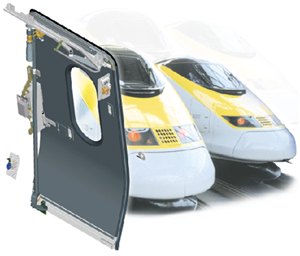
\includegraphics[width=.95\textwidth]{images/fig_01}
\end{center}
\end{minipage}


 	Les performances du TGV (vitesse, confort, proximité des gares) ont conduit à un essor important du trafic de voyageurs. Les opérateurs ferroviaires ont dû par conséquent  adapter le cahier des charges de leurs équipements pour faire face à cette demande accrue. Le matériel voyageur a ainsi subi une évolution et une modernisation sans précédent depuis plusieurs années.
Nous nous intéresserons dans le cadre de ce travail au système « porte » autorisant la communication entre l’intérieur et l’extérieur du train.
}

\subsection{Orientation de l'étude}

\ifthenelse{\boolean{prof}}{}{
Au cours de son cycle de vie, de sa conception à son recyclage, les conditions de fonctionnement du système d’ouverture fermeture évoluent, influençant notablement ses performances. Une observation continue de certains paramètres vitaux est indispensable au bon fonctionnement de ce système. Cette surveillance poursuit un double objectif :
\begin{itemize}
\item à court terme, celui de maintenir des performances compatibles avec celles définies par le cahier des charges;
\item à plus long terme, celui de planifier des opérations de maintenance corrective afin de pallier tout risque de défaillance.
\end{itemize}

On se propose dans cette étude de montrer comment l’observation au cours du cycle de vie de certaines grandeurs caractéristiques du système permet d’atteindre le premier objectif.

Le sujet s’articule selon trois axes ; après avoir présenté l’objet de l’étude puis analysé dans un premier temps le fonctionnement nominal du système considéré, on aborde ensuite l’étude de plusieurs fonctionnalités liées à sa phase courante d’utilisation.

Les exigences liées au système sont données dans le diagramme figure \ref{fig_req}.
\begin{figure}[!ht]
\begin{center}
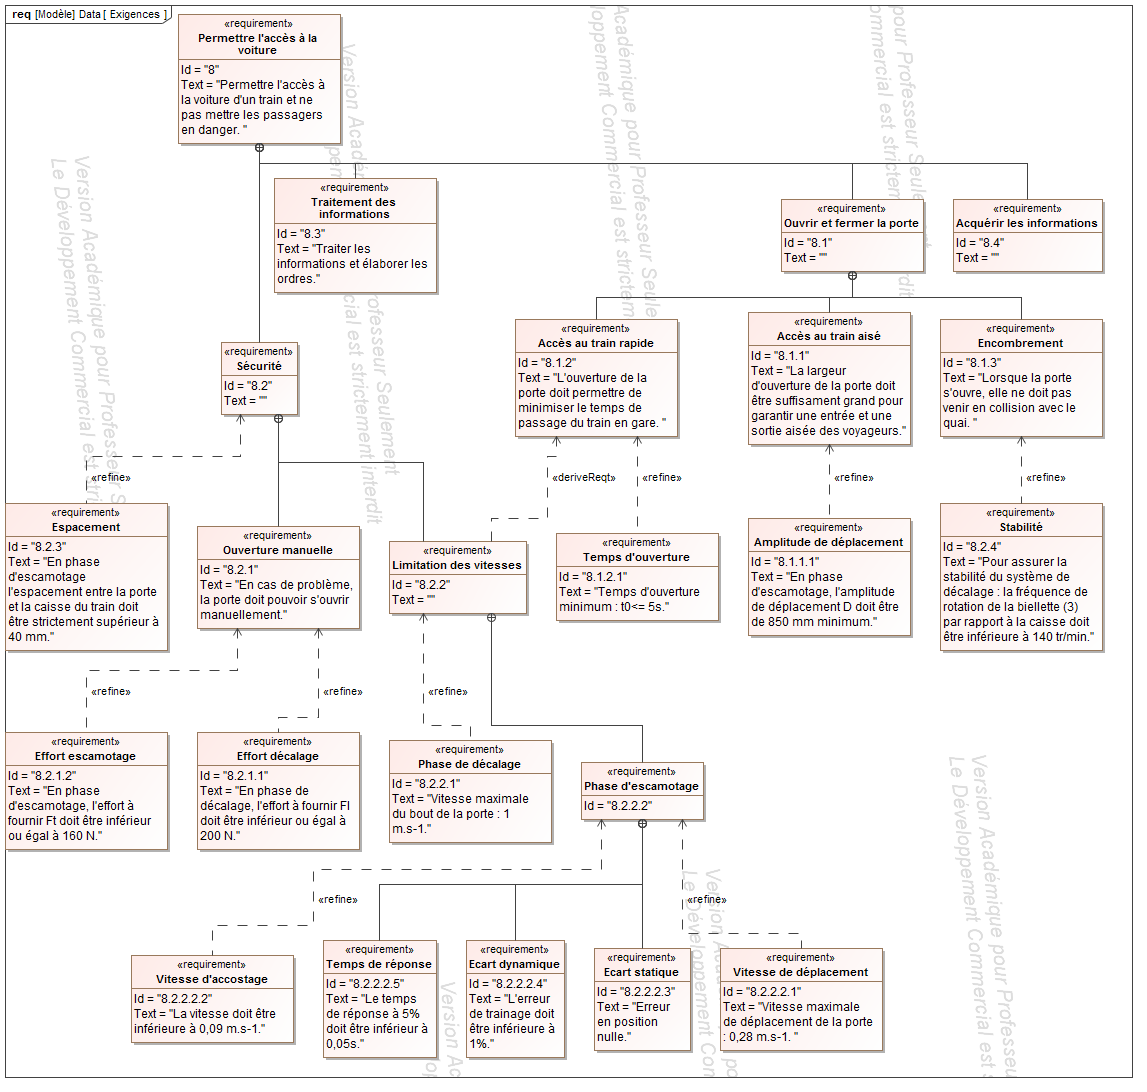
\includegraphics[width=\textwidth]{images/req}

\caption{Diagramme des exigences \label{fig_req}}
\end{center}
\end{figure}
}

\subsection{Présentation du système}

\ifthenelse{\boolean{prof}}{}{
La figure \ref{fig_01} montre l’interface assurant, à partir des informations délivrées par l’unité centrale de commande, la fermeture hermétique et le verrouillage de la porte. L’ordre de fermeture de la porte est donné soit par appui sur le bouton situé sur la porte soit via un ordre fourni par le conducteur depuis son pupitre. L’information est traitée par l’unité centrale qui pilote un moteur électrique permettant, dans un premier temps, de fermer la porte grâce à un mécanisme pignon-crémaillère puis, dans un deuxième temps, lorsque la position de fermeture est détectée, de verrouiller la porte. La détection de la position fermée enclenche également le gonflage des joints assurant l’herméticité de la fermeture. L’information de fin d’opération est transmise au conducteur sur son pupitre.


\begin{figure}[!h]
\begin{center}
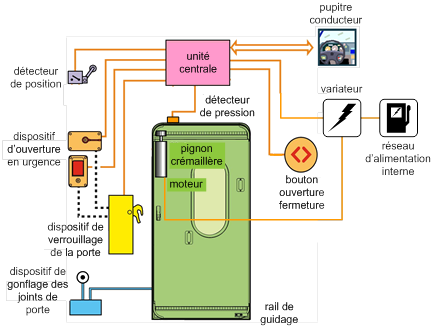
\includegraphics[width=.65\textwidth]{images/fig_02}

\caption{Interface fonctionnelle du système porte \label{fig_01}}
\end{center}
\end{figure}
}

\ifthenelse{\boolean{prof}}{}{\clearpage}

\subparagraph{}
\textit{\`A partir de la figure \ref{fig_01}, compléter le diagramme de blocs sur le document réponse.}
\ifthenelse{\boolean{prof}}{
\begin{corrige}
\begin{center}
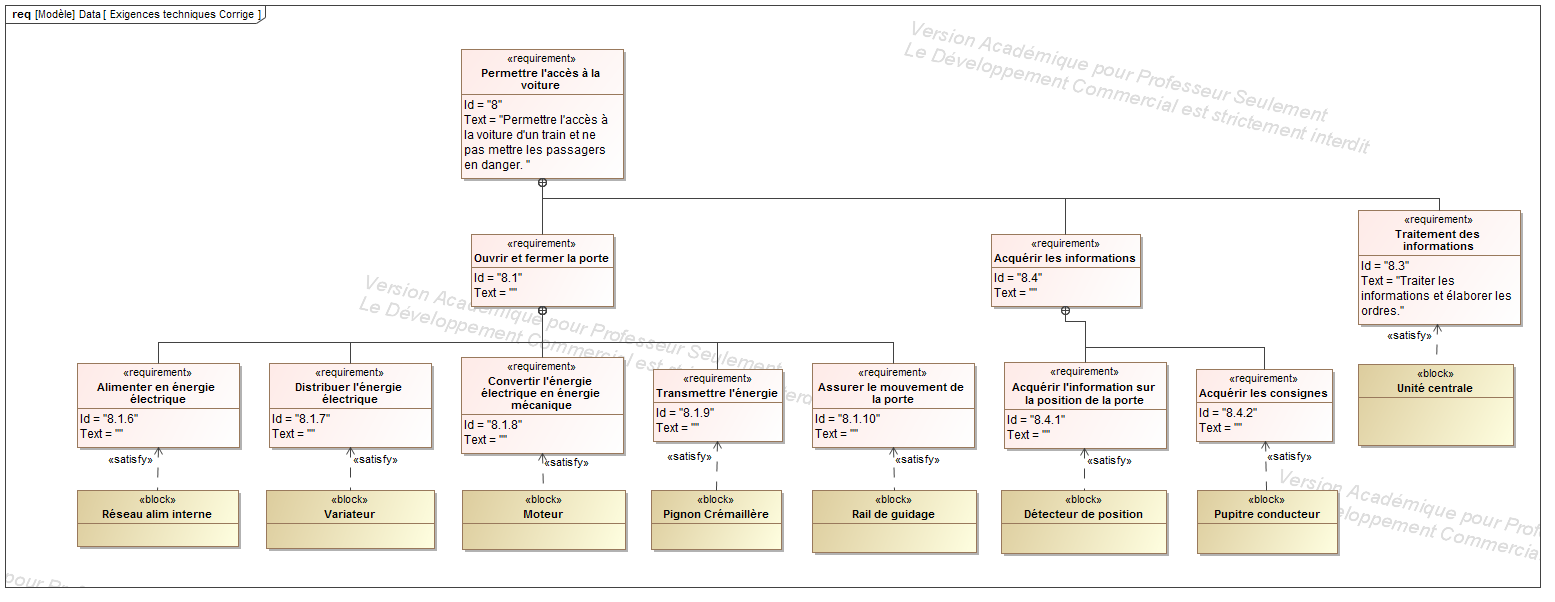
\includegraphics[width=\textwidth]{images/SysML/ExigencesCorrige}
\end{center}
\end{corrige}}{
\begin{center}
\rotatebox{90}{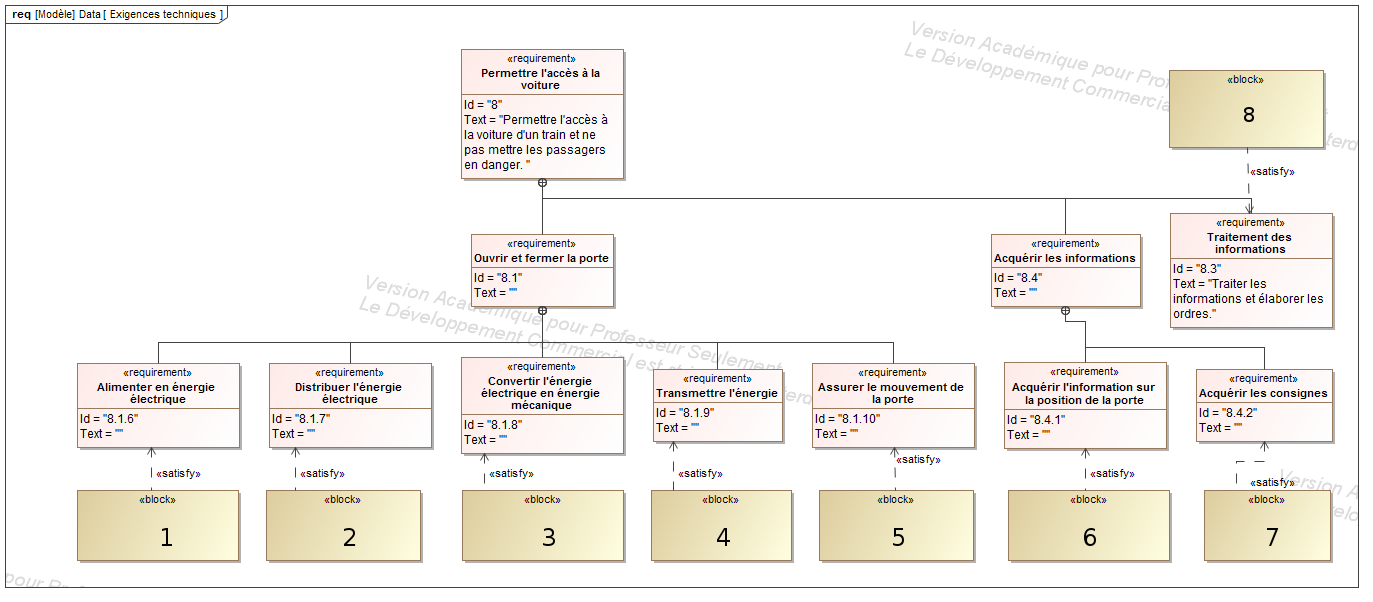
\includegraphics[width=0.95\textheight]{images/SysML/Exigencestechniques2.png}}
\end{center}}

\section{Étude du mouvement de la porte en mode nominal}

\ifthenelse{\boolean{prof}}{}{
\begin{obj}
L’objectif de cette étude est de déterminer les performances de la solution technique implantée sur le TGV pour le mécanisme d’ouverture/fermeture de la porte d’accès et de valider leurs conformités avec les exigences formulées (figure \ref{fig_req}).
\end{obj}

L’architecture et l’implantation de la partie opérative étudiée est précisée sur la figure 2. On y distingue le mécanisme d’ouverture/fermeture (objet de cette étude) dont la fonction est d’assurer l’accès au train en escamotant latéralement le panneau de porte.
\begin{figure}[!h]
\begin{center}
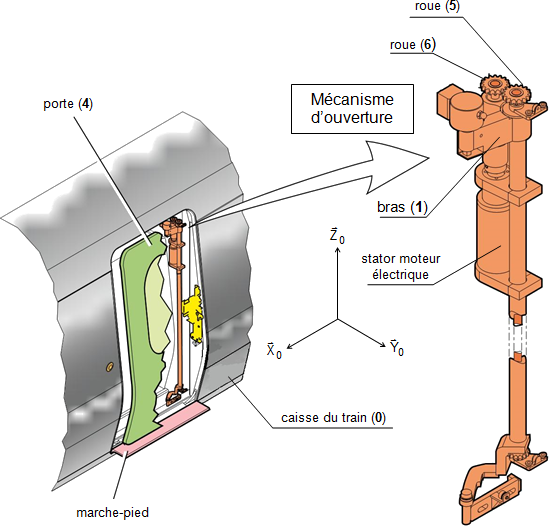
\includegraphics[width=.65\textwidth]{images/fig_03}

\caption{Architecture générale \label{fig_02}}
\end{center}
\end{figure}



Afin de satisfaire les contraintes d’encombrement, l’ouverture de la porte s’effectue selon l’enchaînement temporel de trois phases distinctes décrites à partir de la position <<porte fermée>> pour laquelle la face extérieure de la porte est alignée avec la face extérieure de la caisse ; une phase de décalage puis une phase de louvoiement et enfin une phase d’escamotage. La phase primaire (décalage) puis la phase terminale (escamotage) sont définies par les figures suivantes.
\begin{minipage}[c]{.47\linewidth}
%\begin{figure}[!ht]
\begin{center}
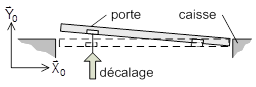
\includegraphics[width=.8\textwidth]{images/fig_04}

\textit{Phase de décalage}% \label{fig_04}}
\end{center}
%\end{figure}

\end{minipage}\hfill
\begin{minipage}[c]{.47\linewidth}
Phase de décalage : ce premier mouvement permet de décaler angulairement la porte (4) de la caisse du wagon.
\end{minipage}

\begin{minipage}[c]{.47\linewidth}
\begin{center}
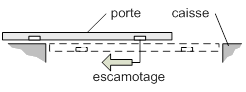
\includegraphics[width=.8\textwidth]{images/fig_05}

\textit{Phase d'escamotage}
\end{center}
\end{minipage}\hfill
\begin{minipage}[c]{.47\linewidth}
Phase d’escamotage : la porte (4) coulisse le long de la caisse du wagon, dégageant ainsi complètement l’accès au train.
\end{minipage}
}

\subparagraph{}
\textit{Décrire en quelques lignes la phase intermédiaire de louvoiement en précisant la nature du mouvement de la porte (4) par rapport à la caisse (0).}
\ifthenelse{\boolean{prof}}{
\begin{corrige}
En première approche, on peut considérer que le mouvement de la porte est une rotation d'axe $\vect{z_0}$. Cette phase a pour but de remettre la porte <<parallèle>> à la caisse.
\end{corrige}}{}


\subparagraph{}
\textit{En le reprenant sur votre feuille, compléter le tableau ci-dessous recensant les degrés de mobilité (nombre et nature) de la porte (4) par rapport à la caisse du TGV (0) lors des différentes phases.}
\ifthenelse{\boolean{prof}}{
\begin{corrige}
\begin{center}
\begin{tabular}{|l|c|c|}
\hline
& Nombre & Nature \\
\hline
\hline
Décalage      & 1 & Rotation \\ \hline
Louvoiement & 1 & Rotation \\ \hline
Escamotage & 1 & Translation\\ \hline
\end{tabular}
\end{center}
\end{corrige}}{}

\ifthenelse{\boolean{prof}}{}{
\begin{center}
\begin{tabular}{|l|c|c|}
\hline
& Nombre & Nature \\
\hline
\hline
Décalage & & \\ \hline
Louvoiement & & \\ \hline
Escamotage & & \\ \hline
\end{tabular}
\end{center}
}

\subsection{Étude analytique de la phase de décalage}

\begin{obj}
Vérifier la satisfaction de l'exigence de 8.2.2.1.
\end{obj}

\ifthenelse{\boolean{prof}}{}{
Le mécanisme d’ouverture de la porte est mis en mouvement grâce à l’action d’un unique moteur électrique (cf. figure \ref{fig_02} et figure \ref{fig_04}). Le rotor de cet actionneur est solidaire de la roue (6) alors que son stator est fixé sur le bras (1). Par commodité, on adopte $\dot{\theta}_{61}(t)=\dot{\theta}_m(t)$ . La roue motrice (6) est par construction en liaison pivot d’axe  $\axe{B}{z_0}$ par rapport au bras (1). La roue (6) entraîne en rotation la roue (5) provoquant alors le mouvement de la porte (4). Un système articulé dit de <<stabilisation>> se composant des biellettes (2) et (3), complète le mécanisme. La biellette (2) est en liaison pivot d’axe $\axe{B}{z_0}$  par rapport au bras (1).

On réduit le problème à une résolution plane et on suppose que la roue (5) roule sans glisser sur la porte (4) et que de la même façon, la roue (5) roule sans glisser sur la roue (6). On pose $\vect{EI(t)}=\lambda(t)\vect{y_4}$.
\begin{figure}[!h]
\begin{center}
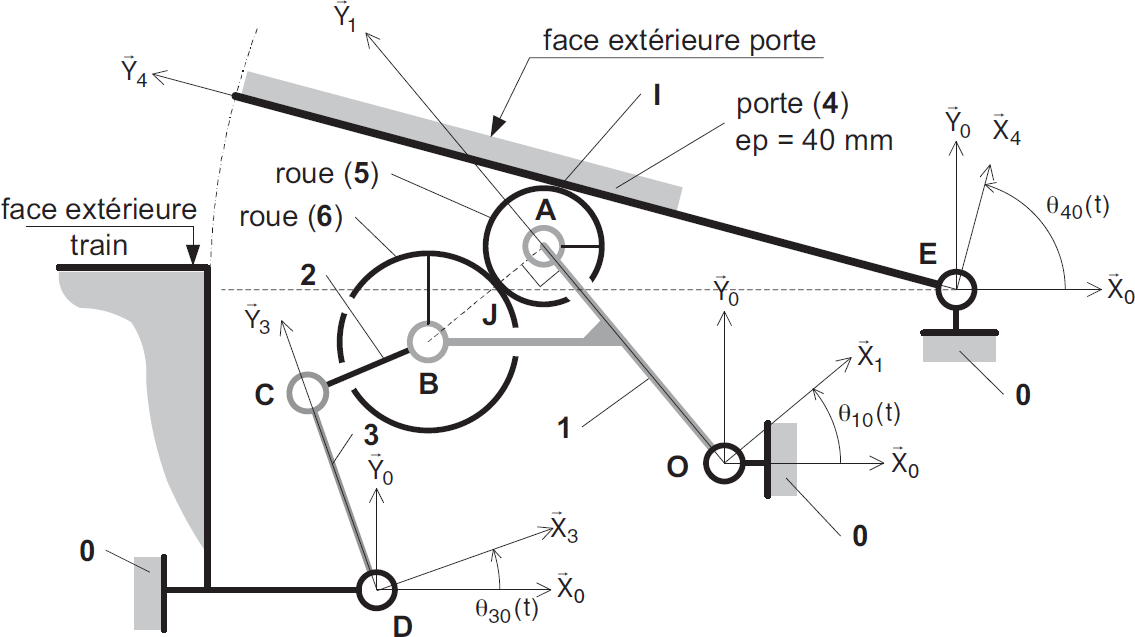
\includegraphics[width=.8\textwidth]{images/fig_06}

\caption{Schéma cinématique plan -- << Phase décalage en cours >> \label{fig_04}}
\end{center}
\end{figure}
}

\subparagraph{}
\textit{Comment varie la longueur EI au cours de la phase de décalage ?}
\ifthenelse{\boolean{prof}}{
\begin{corrige}
Lors de la phase de décalage la longueur EI diminue.
\end{corrige}}{}



\subparagraph{}
\textit{Dans quel sens (horaire ou trigonométrique) doit tourner la roue (6) par rapport au bras (1) afin de provoquer le décalage angulaire de la porte (4) par rapport à la caisse (0) ?}
\ifthenelse{\boolean{prof}}{
\begin{corrige}
La roue (6) doit tourner dans le sens horaire pour provoquer le décalage angulaire de la porte par rapport à la caisse. 
\end{corrige}}{}

\ifthenelse{\boolean{prof}}{}{
\begin{hypo}
\textbf{Hypothèses :}
\begin{itemize}
\item Les liaisons pivot sont modélisées comme étant parfaites.
\item Le repère $\rep{0}{O}{x_0}{y_0}{z_0}$ lié au support (0) est considéré comme galiléen, l’axe $\axe{O}{z_0}$ étant vertical ascendant.
\item le repère  $\rep{1}{O}{x_1}{y_1}{z_0}$ est lié au bras (1). Ce dernier (qui supporte les deux roues (5 et 6) est animé d’un mouvement de rotation autour de l’axe  $\axe{O}{z_0}$. On pose : $\theta_{10}(t)=\left( \vect{x_0},\vect{x_1}\right)$.
\item Le repère  $\rep{2}{C}{x_2}{y_2}{z_0}$ est lié à la biellette de réaction (2). On pose :  $\theta_{20}(t)=\left( \vect{x_0},\vect{x_2}\right)$.
\item Le repère $\rep{3}{D}{x_3}{y_3}{z_0}$  est lié à la biellette (3). Cette dernière est animée d’un mouvement de rotation autour de l’axe  $\axe{D}{z_0}$. On pose $\theta_{30}(t)=\left( \vect{x_0},\vect{x_3}\right)$.
\item Le repère $\rep{4}{E}{x_4}{y_4}{z_0}$  est lié à la porte (4). On pose $\theta_{40}(t)=\left( \vect{x_0},\vect{x_4}\right)$. Porte fermée : $\theta_{40}(t=0)=90\textdegree$.
\item On note $\theta_{51}$ l'angle de rotation de la roue (5) par rapport au bras (1).
\item La roue (5) roule sans glisser sur la porte (4) en $I$ et sur la roue (6) en $J$.  
\end{itemize}


\textbf{Caractéristiques géométriques :}
\begin{itemize}
\item Bâti (0) :
\begin{itemize}
\item $\vect{DO}=L\vect{x_0} + H\vect{y_0}$ avec $L=190\; mm$ et $H=60\; mm$;
\item $\vect{OE}=L_0\vect{x_0} + H_0\vect{y_0}$ avec $L_0=544\; mm$ et $H_0=65,8\; mm$.
\end{itemize}
\item Biellette (3) : $\vect{DC}=L_3\vect{y_3}$ avec $L_3 = 88\; mm$.
\item Biellette (2) : $\vect{CB}=L_2\vect{x_2}$ avec $L_2 = 62,6\; mm$.
\item Bras support (1) : 
\begin{itemize}
\item $\vect{OA}=L_1\vect{y_1}$ avec $L_1 = 149\; mm$;
\item $\vect{AB}=-\left( R_5+R_6\right)\vect{x_1}$;
\item masse : $m_1 = 13,4\; kg$.
\end{itemize}
\item Porte (4) : 
\begin{itemize}
\item largeur : $L_4 = 850 \; mm$;
\item épaisseur moyenne : $40\; mm$;
\item masse : $m_3 = 120\; kg$.
\end{itemize}
\item Roue (5) : 
\begin{itemize}
\item rayon : $R_5 = 29\; mm$;
\item masse : $m_5$.
\end{itemize}
\item Roue (6) + rotor du moteur à courant continu : 
\begin{itemize}
\item rayon : $R_6 = 37\; mm$;
\item masse : $m_6$.
\end{itemize}
\end{itemize}
\end{hypo}

}

\subparagraph{\label{ferm_geo}}
\textit{Écrire l'équation de fermeture géométrique liée à la boucle fermée constituée de la chaîne de solides 0 -- 1 -- 5 -- 4.}

\subparagraph{}
\textit{Déterminer alors la loi entrée sortie en exprimant $\theta_{40}$ en fonction de $\theta_{10}$. Pour cela on mettra l'expression sous la forme $\sin\theta_{40}\cdot f(\theta_{10})+\cos\theta_{40}\cdot g(\theta_{10})=1$ où $f$ et $g$ sont des fonctions à déterminer. }
\ifthenelse{\boolean{prof}}{
\begin{corrige}
On a :
$$
\vect{OA} + \vect{AI}+\vect{IE}+\vect{EO}=\vect{0}
\quad
L_1\vect{y_1} + R_5 \vect{x_4} + \lambda(t) \vect{y_4} -L_0\vect{x_0}-H_0\vect{y_0}=\vect{0}
$$

En projetant cette équation sur $\vect{x_0}$ :
$$
-L_1\sin\theta_{10} + R_5\cos\theta_{40} - \lambda(t) \sin\theta_{40} -L_0 = 0 \Longleftrightarrow 
\lambda(t) = \dfrac{-L_1\sin\theta_{10} + R_5\cos\theta_{40}  -L_0}{\sin\theta_{40}}
$$

En projetant cette équation sur $\vect{y_0}$ :
$$
L_1\cos\theta_{10} + R_5\sin\theta_{40} + \lambda(t) \cos\theta_{40} -H_0 = 0
\Longleftrightarrow 
\lambda(t) = \dfrac{-L_1\cos\theta_{10} - R_5\sin\theta_{40} +H_0 }{\cos\theta_{40}}
$$

On a donc : 
$$
\dfrac{-L_1\sin\theta_{10} + R_5\cos\theta_{40}  -L_0}{\sin\theta_{40}}
= 
\dfrac{-L_1\cos\theta_{10} - R_5\sin\theta_{40} +H_0 }{\cos\theta_{40}}
$$
$$
\Longleftrightarrow
-L_1\sin\theta_{10}\cos\theta_{40} + R_5\cos^2\theta_{40} - L_0\cos\theta_{40}
=
-L_1\cos\theta_{10}\sin\theta_{40} - R_5\sin^2\theta_{40} +H_0\sin\theta_{40}
$$
$$
\Longleftrightarrow
\cos\theta_{40}\left(-L_1\sin\theta_{10} - L_0\right) + R_5
=
\sin\theta_{40}\left(-L_1\cos\theta_{10} +H_0\right)
$$
$$
\Longleftrightarrow
\sin\theta_{40}\left(-L_1\cos\theta_{10} +H_0\right)-\cos\theta_{40}\left(L_1\sin\theta_{10} + L_0\right) = R_5
$$

\end{corrige}}{}


\subparagraph{}
\textit{Exprimer chacun des torseurs des liaisons entrant en compte dans la chaîne de solides 0 -- 1 -- 5 -- 4 au point $I$.}
\ifthenelse{\boolean{prof}}{
\begin{corrige}
Liaison 1 -- 0 : pivot de centre $O$ :
$$
\torseurcin{V}{1}{0}
=\torseurl{\vecto{1}{0}=\dot{\theta}_{10}\vect{z_0}}{\vectv{O}{1}{0}=\vect{0}}{O}
=\torseurl{\vecto{1}{0}=\dot{\theta}_{10}\vect{z_0}}{\vectv{I}{1}{0}=}{I}
$$

$$
\vectv{I}{1}{0}
=\vectv{O}{1}{0}+ \vect{IO}\wedge\vecto{1}{0}
=\left( -R_5 \vect{x_4} -L_1\vect{y_1} \right)\wedge \dot{\theta}_{10}\vect{z_0}
= R_5 \dot{\theta}_{10}\vect{y_4} -L_1 \dot{\theta}_{10}\vect{x_1}
$$

$$
\torseurcin{V}{1}{0}
=\torseurl{\vecto{1}{0}=\dot{\theta}_{10}\vect{z_0}}{\vectv{I}{1}{0}=R_5 \dot{\theta}_{10}\vect{y_4} -L_1 \dot{\theta}_{10}\vect{x_1}}{I}
$$

Liaison 5 -- 1 : pivot de centre $A$ :
$$
\torseurcin{V}{5}{1}
=\torseurl{\vecto{5}{1}=\dot{\theta}_{51}\vect{z_0}}{\vectv{A}{5}{1}=\vect{0}}{A}
=\torseurl{\vecto{5}{1}=\dot{\theta}_{51}\vect{z_0}}{\vectv{I}{5}{1}=}{I}
$$

$$
\vectv{I}{5}{1}
=\vectv{A}{5}{1}+ \vect{IA}\wedge\vecto{5}{1}
=-R_5 \vect{x_4} \wedge \dot{\theta}_{51}\vect{z_0}
= R_5 \dot{\theta}_{51}\vect{y_4}
$$

$$
\torseurcin{V}{5}{1}
=\torseurl{\vecto{5}{1}=\dot{\theta}_{51}\vect{z_0}}{\vectv{I}{5}{1}=R_5 \dot{\theta}_{51}\vect{y_4}}{I}
$$


Liaison 4 -- 5 : contact sphère -- cylindre avec roulement sans glissement en $I$ :
$$
\torseurcin{V}{4}{5}
=\torseurl{\vecto{4}{5}=\dot{\theta}_{45}\vect{z_0}}{\vectv{I}{4}{5}=\vect{0}}{I}
$$

Liaison 4 -- 0 : pivot de centre $E$ :
$$
\torseurcin{V}{4}{0}
=\torseurl{\vecto{4}{0}=\dot{\theta}_{40}\vect{z_0}}{\vectv{A}{4}{0}=\vect{0}}{E}
=\torseurl{\vecto{4}{0}=\dot{\theta}_{40}\vect{z_0}}{\vectv{I}{4}{0}=}{I}
$$

$$
\vectv{I}{4}{0}
=\vectv{E}{4}{0}+ \vect{IE}\wedge\vecto{4}{0}
=\lambda(t) \vect{y_4} \wedge \dot{\theta}_{40}\vect{z_0}
= \lambda(t) \dot{\theta}_{40}\vect{x_4}
$$

$$
\torseurcin{V}{4}{0}
=\torseurl{\vecto{4}{0}=\dot{\theta}_{40}\vect{z_0}}{\vectv{I}{4}{0}=\lambda(t) \dot{\theta}_{40}\vect{x_4}}{I}
$$
\end{corrige}}

\subparagraph{}
\textit{Réaliser la fermeture de chaîne cinématique au point $I$. On projettera l'équation des vecteurs vitesse dans la base $\mathcal{R}_4$.}

\ifthenelse{\boolean{prof}}{
\begin{corrige}
La fermeture de chaîne cinématique donne : 
$$
\torseurcin{V}{4}{5}+\torseurcin{V}{5}{1}+\torseurcin{V}{1}{0} = \torseurcin{V}{4}{0}
$$

La fermeture des vecteur instantané de rotation se traduit par : 
$$
 \dot{\theta}_{45}\vect{z_0}  + \dot{\theta}_{51}\vect{z_0}  + \dot{\theta}_{10}\vect{z_0} 
= \dot{\theta}_{40}\vect{z_0}
\Longrightarrow 
 \dot{\theta}_{45} + \dot{\theta}_{51}  + \dot{\theta}_{10}= \dot{\theta}_{40}
$$

La fermeture des vecteurs vitesse donne :
$$
\vect{0}
+R_5 \dot{\theta}_{51}\vect{y_4}
+R_5 \dot{\theta}_{10}\vect{y_4} -L_1 \dot{\theta}_{10}\vect{x_1}
=\lambda(t) \dot{\theta}_{40}\vect{x_4}
\Longleftrightarrow 
R_5 \dot{\theta}_{51}\vect{y_4}
+R_5 \dot{\theta}_{10}\vect{y_4} -L_1 \dot{\theta}_{10}\vect{x_1}
=\lambda(t) \dot{\theta}_{40}\vect{x_4}
$$

Exprimons $\vect{x_1}$ dans le repère $\mathcal{R}_4$ : 
$$
\vect{x_1}= \cos\theta_{10}\vect{x_0} + \sin\theta_{10}\vect{y_0}
\quad \quad 
\vect{x_0}= \cos\theta_{40}\vect{x_4} - \sin\theta_{40}\vect{y_4}
\quad\quad 
\vect{y_0}= \cos\theta_{40}\vect{y_4} + \sin\theta_{40}\vect{x_4}
$$

On a donc :
$$
\vect{x_1}= \cos\theta_{10}\left(\cos\theta_{40}\vect{x_4} - \sin\theta_{40}\vect{y_4} \right)+ \sin\theta_{10}\left( \cos\theta_{40}\vect{y_4} + \sin\theta_{40}\vect{x_4}\right)
$$

$$
\Longleftrightarrow 
\vect{x_1}= \left(\cos\theta_{10}\cos\theta_{40}+ \sin\theta_{10}\sin\theta_{40} \right)\vect{x_4} + \left( \sin\theta_{10}\cos\theta_{40}-\cos\theta_{10} \sin\theta_{40}\right)\vect{y_4} 
$$
$$
\Longleftrightarrow 
\vect{x_1}= \cos\left(\theta_{10}-\theta_{40} \right)\vect{x_4} 
+ \sin\left(\theta_{10}-\theta_{40} \right)\vect{y_4} 
$$

On a alors : 

$$
R_5 \dot{\theta}_{51}\vect{y_4}
+R_5 \dot{\theta}_{10}\vect{y_4} -L_1 \dot{\theta}_{10}\left(\cos\left(\theta_{10}-\theta_{40} \right)\vect{x_4} 
+ \sin\left(\theta_{10}-\theta_{40} \right)\vect{y_4}  \right)
=\lambda(t) \dot{\theta}_{40}\vect{x_4}
$$
En projetant sur $\vect{x_4}$ et sur $\vect{y_4}$ : 
$$
 -L_1 \dot{\theta}_{10}\cos\left(\theta_{10}-\theta_{40} \right)
=\lambda(t) \dot{\theta}_{40}
$$
$$
R_5 \dot{\theta}_{51}
+R_5 \dot{\theta}_{10}
-L_1 \dot{\theta}_{10}\sin\left(\theta_{10}-\theta_{40} \right)
=0
$$
\end{corrige}}{}



\subparagraph{}
\textit{Calculer $\vectv{A}{5}{4}$ par le calcul direct.}
\ifthenelse{\boolean{prof}}{
\begin{corrige}
$$
\vectv{A}{5}{4} 
= \left[\dfrac{d\vect{EA}}{dt}\right]_{\mathcal{R}_4}
= \left[\dfrac{d\vect{EI}}{dt}\right]_{\mathcal{R}_4}+\left[\dfrac{d\vect{IA}}{dt}\right]_{\mathcal{R}_4}
= \left[\dfrac{d-\lambda(t)\vect{y_4}}{dt}\right]_{\mathcal{R}_4}+\left[\dfrac{d-R_5\vect{x_4}}{dt}\right]_{\mathcal{R}_4}
= -\dot{\lambda}(t)\vect{y_4}
$$

\end{corrige}}{}



\subparagraph{}
\textit{\`A partir de la condition de roulement sans glissement au point $I$, déterminer une deuxième expression de $\vectv{A}{5}{4}$ à l'aide du champ des vitesses. En déduire une relation scalaire liant $\dot{\lambda}$, $R_5$ et $\dot{\theta}_{54}$.}
\ifthenelse{\boolean{prof}}{
\begin{corrige}
$$
\vectv{A}{5}{4} 
= \vectv{I}{5}{4} +  \vect{AI}\wedge \vecto{5}{4}
=R_5\vect{x_4} \wedge \dot{\theta}_{54}\vect{z_0}
=-R_5\dot{\theta}_{54} \vect{y_4}
$$

En utilisant la question précédente, on a alors : 
$$
 -\dot{\lambda}(t)\vect{y_4}=-R_5\dot{\theta}_{54} \vect{y_4}
 \Longrightarrow 
  \dot{\lambda}(t)=R_5\dot{\theta}_{54}
$$
\end{corrige}}{}


\subparagraph{}
\textit{Montrer que l'équation vectorielle obtenue par la fermeture cinématique correspond à l'équation vectorielle dérivée issue de la fermeture de géométrique de la question \ref{ferm_geo}.}
\ifthenelse{\boolean{prof}}{
\begin{corrige}
En utilisant la fermeture cinématique on a : 
$$R_5 \dot{\theta}_{51}\vect{y_4}
+R_5 \dot{\theta}_{10}\vect{y_4} -L_1 \dot{\theta}_{10}\left(\cos\left(\theta_{10}-\theta_{40} \right)\vect{x_4} 
+ \sin\left(\theta_{10}-\theta_{40} \right)\vect{y_4}  \right)
=\lambda(t) \dot{\theta}_{40}\vect{x_4}
$$

En utilisant la fermeture géométrique, on a : 
$$L_1\vect{y_1} + R_5 \vect{x_4} + \lambda(t) \vect{y_4} -L_0\vect{x_0}-H_0\vect{y_0}=\vect{0}
$$

En dérivant l'expression on obtient donc : 
$$-L_1\dot{\theta}_{10}\vect{x_1} + R_5 \dot{\theta}_{40}\vect{y_4} + \dot{\lambda}(t) \vect{y_4} - \lambda(t)\dot{\theta}_{40}\vect{x_4}=\vect{0}
\Longleftrightarrow
-L_1\dot{\theta}_{10}\vect{x_1} + R_5 \dot{\theta}_{40}\vect{y_4} +
\dot{\lambda}(t) \vect{y_4}=
 \lambda(t)\dot{\theta}_{40}\vect{x_4}
$$
$$
\Longleftrightarrow
-L_1\dot{\theta}_{10}\left( 
\cos\left(\theta_{10}-\theta_{40} \right)\vect{x_4} 
+ \sin\left(\theta_{10}-\theta_{40} \right)\vect{y_4} 
\right) + R_5 \dot{\theta}_{40}\vect{y_4} +
\dot{\lambda}(t) \vect{y_4}=
 \lambda(t)\dot{\theta}_{40}\vect{x_4}
$$

Il faut donc montrer que : 
$R_5 \dot{\theta}_{51}\vect{y_4}
+R_5 \dot{\theta}_{10}\vect{y_4} = R_5 \dot{\theta}_{40}\vect{y_4} +
\dot{\lambda}(t) \vect{y_4} \Longrightarrow
\dot{\theta}_{51} + \dot{\theta}_{10} = \dot{\theta}_{40} +
\dot{\theta}_{54} $. 

Or, d'après la fermeture cinématique, on a vu que :
$$
\dot{\theta}_{45} + \dot{\theta}_{51}  + \dot{\theta}_{10}= \dot{\theta}_{40}
\Longleftrightarrow
 \dot{\theta}_{51}  + \dot{\theta}_{10}= \dot{\theta}_{40} + \dot{\theta}_{54} 
$$
\textit{CQFD.}

%$$
%\Longrightarrow  R_5 \dot{\theta}_{10}\vect{y_4} + R_5 \dot{\theta}_{51}\vect{y_4}
%+  R_5 \dot{\theta}_{41}\vect{y_4} + R_5 \dot{\theta}_{51}\vect{y_4}
%\left(\dot{\theta}_{41}+\right)
%+ R_5\left(\dot{\theta}_{51}+\dot{\theta}_{14}(t)\right) \vect{y_4}
%$$


\end{corrige}}{}



Les courbes 1 et 2 présentent les évolutions obtenues par simulation numérique de la position angulaire de la porte $\theta_{40}$, de la position angulaire du bras support (1) $\theta_{10}$ et du rapport $\dfrac{\theta_{40}}{\theta_{10}}$ en fonction de l’angle de rotation du moteur $\theta_{61}$.
On suppose qu’à l’instant initial $t=0$, on se trouve dans la configuration <<porte fermée>> pour laquelle on considère que $\theta_{61}=\theta_{51}=0$.

\begin{minipage}[c]{.48\linewidth}
\begin{center}
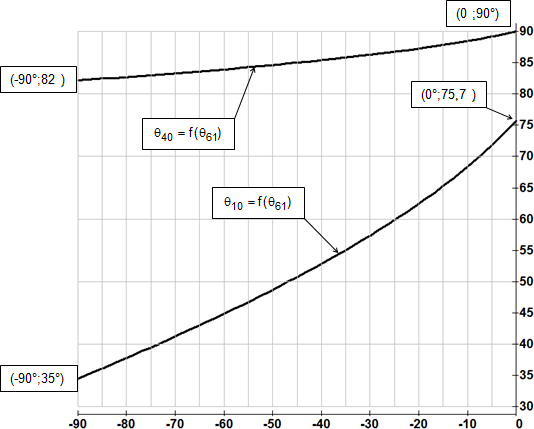
\includegraphics[width=\textwidth]{images/ann_2_1}

\textit{Courbe 1 -- Évolutions (en $\textdegree$) de $\theta_{40}=f(\theta_{61})$ et  $\theta_{10}=f(\theta_{61})$}
\end{center}
\end{minipage} \hfill
\begin{minipage}[c]{.48\linewidth}
\begin{center}
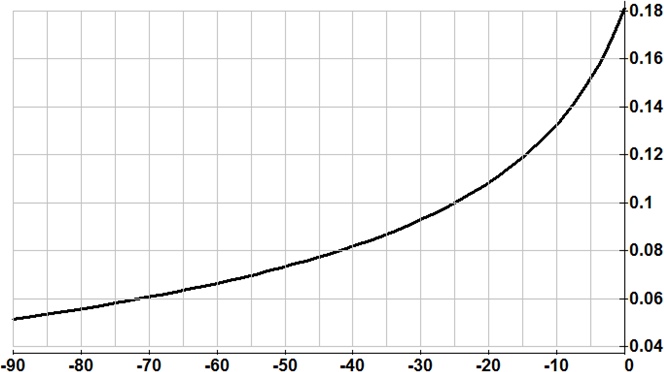
\includegraphics[width=\textwidth]{images/ann_2_2}

\textit{Courbe 2 -- Évolution de $\dfrac{\dot{\theta}_{40}}{\dot{\theta}_{61}}=f(\theta_{61})$}
\end{center}
\end{minipage} 
\subparagraph{}
\textit{A l'aide des équations scalaires obtenues grâce à la fermeture géométrique et de la courbe 1 faire l'application numérique pour la configuration $t=0\; s$ afin de déterminer le rayon $R_5$ ainsi que la valeur de $\lambda(t=0)$ notée $\lambda_0$.($\cos 75,7 \simeq 0,25$ et $\sin 75,7 \simeq 0,97$ )}
\ifthenelse{\boolean{prof}}{
\begin{corrige}
Les équations scalaires sont les suivantes : 
$$
\lambda(t)\sin\theta_{40} = -L_1\sin\theta_{10} + R_5\cos\theta_{40}  -L_0
\quad \quad 
\lambda(t)\cos\theta_{40} = -L_1\cos\theta_{10} - R_5\sin\theta_{40} +H_0 
$$

En $t=0$, $\theta_{40} = 90\textdegree$ :
$$
\lambda_0\sin\theta_{40} = -L_1\sin\theta_{10}  -L_0 \quad \quad 
0 = -L_1\cos\theta_{10} - R_5 +H_0 
$$

On a donc $R_5 = H_0-L_1\cos\theta_{10} \Longrightarrow R_5 =65,8 -  149\cdot \cos 75,7 \simeq 29\; mm $.

Par ailleurs : 
$\lambda_0 = -L_1\sin\theta_{10}  -L_0 = -149 \sin 75,7 - 544 \simeq 693 \; mm $. 


\end{corrige}}{}


\subparagraph{}
\textit{Déterminer la fréquence de rotation supposée constante du moteur (en $tr/min$) si la durée de la phase de décalage est limitée à 0,3 s.}
\ifthenelse{\boolean{prof}}{
\begin{corrige}
Durant la phase de décalage, la courbe 1 indique que le moteur tourne de 90 degrés. Pour que cette phase soit limitée à 0,3 s, on a donc une vitesse de rotation de 1 tour pour 1,2 s soientt 50 tours par minute. 
\end{corrige}}{}


\subparagraph{}
\textit{En utilisant la courbe 2, déterminer alors la plage de variation de la fréquence de rotation de la porte (4) par rapport à la caisse (0) sachant que la porte a une longueur $L_4=850\; mm$ et une épaisseur $e_4 = 40\; mm$. Conclure vis-à-vis du cahier des charges fonctionnel.}
\ifthenelse{\boolean{prof}}{
\begin{corrige}
On a :
$$
0,05<\dfrac{\dot{\theta}_{40}}{\dot{\theta}_{61}}<0,18 
\Longleftrightarrow
0,05\dot{\theta}_{61}<\dot{\theta}_{40}<0,18\dot{\theta}_{61} 
\Longleftrightarrow
2,5\; tr/min <\dot{\theta}_{40}<9 tr/min
$$

La vitesse maximale en bout de porte est donc de l'ordre de $850\cdot \dfrac{9\cdot 2\pi}{60}\simeq 850 mm/s$. Cela est compatible avec l'exigence 8.2.2.1.
\end{corrige}}{}



%\subparagraph{}
%\textit{
%\begin{itemize}
%\item En utilisant la courbe 1 et la valeur initiale de $\theta_{40}(t=0)=\theta^i_{40}$, extraire la valeur initiale de $\theta_{10}(t=0)=\theta^i_{10}$. Déterminer alors l’expression de $\lambda_0=\lambda(t=0)$  en fonction de $L_1$,  $L_0$ et $\theta^i_{10}$. Faire l’application numérique.
%\item En utilisant les conditions de roulement sans glissement, montrer que  $\lambda(t)=a\theta_{61}(t)+\lambda_0$, $a\in \mathbb{R}$. Déterminer l’expression de la constante $a$.
%\end{itemize}}
%
%\subparagraph{}
%\textit{
%\begin{itemize}
%\item Déterminer la fréquence de rotation supposée constante du moteur (en $tr\cdot min^{-1}$) si la durée de la phase de décalage est limitée à $0,3\;s$.
%\item Déterminer alors en utilisant la courbe 2, la plage de variation de la fréquence de rotation de la porte (4) par rapport à la caisse (0) en $rad\cdot s^{-1}$.
%\item En se plaçant dans la position correspondante, déterminer la norme maximale (en $m\cdot s^{-1}$) de la vitesse en bout de porte (4) par rapport à la caisse (0). Valider le critère du cahier des charges fonctionnel correspondant.
%\end{itemize}}

\subsection{Étude graphique de la phase de décalage}
\ifthenelse{\boolean{prof}}{}{
Afin de satisfaire des contraintes de stabilité, il est nécessaire de limiter la fréquence de rotation   $\dot{\theta}_{30}$ de la biellette (3) lors du tout début de la phase de décalage. On fait l’hypothèse simplificatrice que la fréquence de rotation, imposée par le choix du moteur est égale à $\dot{\theta}_{61}=-50\; tr/min$ (sens horaire). Pour les questions suivantes, on utilisera le document-réponse fourni. On apportera une attention particulière à la qualité des tracés et au respect de l’échelle donnée. L’utilisation de la couleur est fortement conseillée.
}

\subparagraph{}
\textit{Sur le document-réponse fourni, définir géométriquement la position des points (B, C, I, J) dans la configuration <<porte fermée>>. Faire apparaître la roue (6) et les solides (3), (2) et (1).}
\ifthenelse{\boolean{prof}}{
\begin{corrige}
\end{corrige}}{}

Pour la question suivante, on précisera les directions des différentes vitesses et/ou la position des centres instantanés de rotation. On respectera l’échelle des vitesses donnée sur le document réponse. Les justifications des tracés seront reportées directement sur le document-réponse.


\subparagraph{}
\textit{Sur le document-réponse fourni, construire graphiquement la vitesse du point $I$ appartenant à la porte (4) par rapport à (1), soit $\vectv{I}{4}{1}$ à partir de la vitesse $\vectv{J}{6}{1}$. Justifier vos hypothèses. Construire alors les vitesses $\vectv{I}{4}{0}$ et $\vectv{I}{1}{0}$.}

\ifthenelse{\boolean{prof}}{
\begin{corrige}
Le mouvement de (6) par rapport à (1) est une rotation de centre $B$. $\vectv{J}{6}{1}$ est donc tangent au cercle de centre $B$ et de rayon $BJ$. Par ailleurs $\dot{\theta}_{61}=-50\; tr/min$ et $R_6 = 37\; mm$. On a donc $||\vectv{J}{6}{1}||=\dfrac{50\cdot 2\pi}{60}R_6 \simeq 185 \; mm/s$. La rotation dans le sens horaire impose le sens du vecteur. 

Par ailleurs le roulement sans glissement en $J$ entre 6 et 5 impose que $\vectv{J}{6}{1} = \vectv{J}{5}{1}$. On connait donc la norme de 
$\vectv{I}{5}{1}$. Sa direction est perpendiculaire à (AI). La rotation dans le sens trigonométrique de la pièce 5 impose le sens de $\vectv{I}{5}{1}$.


En outre, le roulement sans glissement en $I$ impose que $\vectv{I}{5}{1}=\vect{0}$. En conséquence, 
$\vectv{I}{5}{4} = \vect{0} = \vectv{I}{5}{1}+\vectv{I}{1}{0}+\vectv{I}{0}{4}$ et donc 
$\vectv{I}{4}{0} = \vectv{I}{5}{1}+\vectv{I}{1}{0}$. $\vectv{I}{4}{0}$ est suivant $\vect{x_0}$. $\vectv{I}{5}{1}$ est connu. 
 Le second  Il est donc possible de tracer $\vectv{I}{4}{0}$. 


Enfin, le mouvement de 1 par rapport à 0 est une rotation de centre O. $\vectv{I}{1}{0}$ est donc perpendiculaire à (OI).


\end{corrige}}{}


\subparagraph{}
\textit{Après avoir construit la vitesse $\vectv{B}{1}{0}$, déterminer $\vectv{C}{3}{0}$. En déduire la valeur de $\dot{\theta}_{30}$ en $ rad\cdot s^{-1}$. Valider le critère du cahier des charges fonctionnel correspondant.}

\ifthenelse{\boolean{prof}}{
\begin{corrige}
$O$ est le CIR du mouvement de 1/0 donc $\vectv{B}{1}{0}$ est perpendiculaire à la droite $(OB)$. Par équiprojectivité on a alors 
$\vectv{B}{1}{0}\cdot{\vect{IB}}=\vectv{I}{1}{0}\cdot{\vect{IB}}$.


D'une part, $\vectv{C}{3}{0}=\vectv{C}{3}{2}+\vectv{C}{2}{0}=\vectv{C}{2}{0}$; donc $\vectv{C}{2}{0}$ est perpendiculaire à $(CD)$. D'autre part $\vectv{B}{1}{0}=\vectv{B}{1}{2}+\vectv{B}{2}{0}=\vectv{B}{2}{0}$. On peut donc tracer $\vectv{C}{2}{0}$ par équiprojectivité : 
$\vectv{C}{2}{0}\cdot{\vect{CB}}=\vectv{B}{2}{0}\cdot{\vect{CB}}$.

Graphiquement on obtient $||\vectv{C}{3}{0}||=96\; cm/s$.

Au final : $\dot{\theta}_{30} = \dfrac{||\vectv{C}{3}{0}||}{L_3} = \dfrac{960}{88}\simeq 11 \; rad/s \simeq 11 \dfrac{60}{2\pi}\simeq 110 \; tr/min < 140 \; tr/min$.

L'exigence 8.2.4 est satisfaite.
\end{corrige}}{}

\ifthenelse{\boolean{prof}}{
\begin{center}
\rotatebox{90}{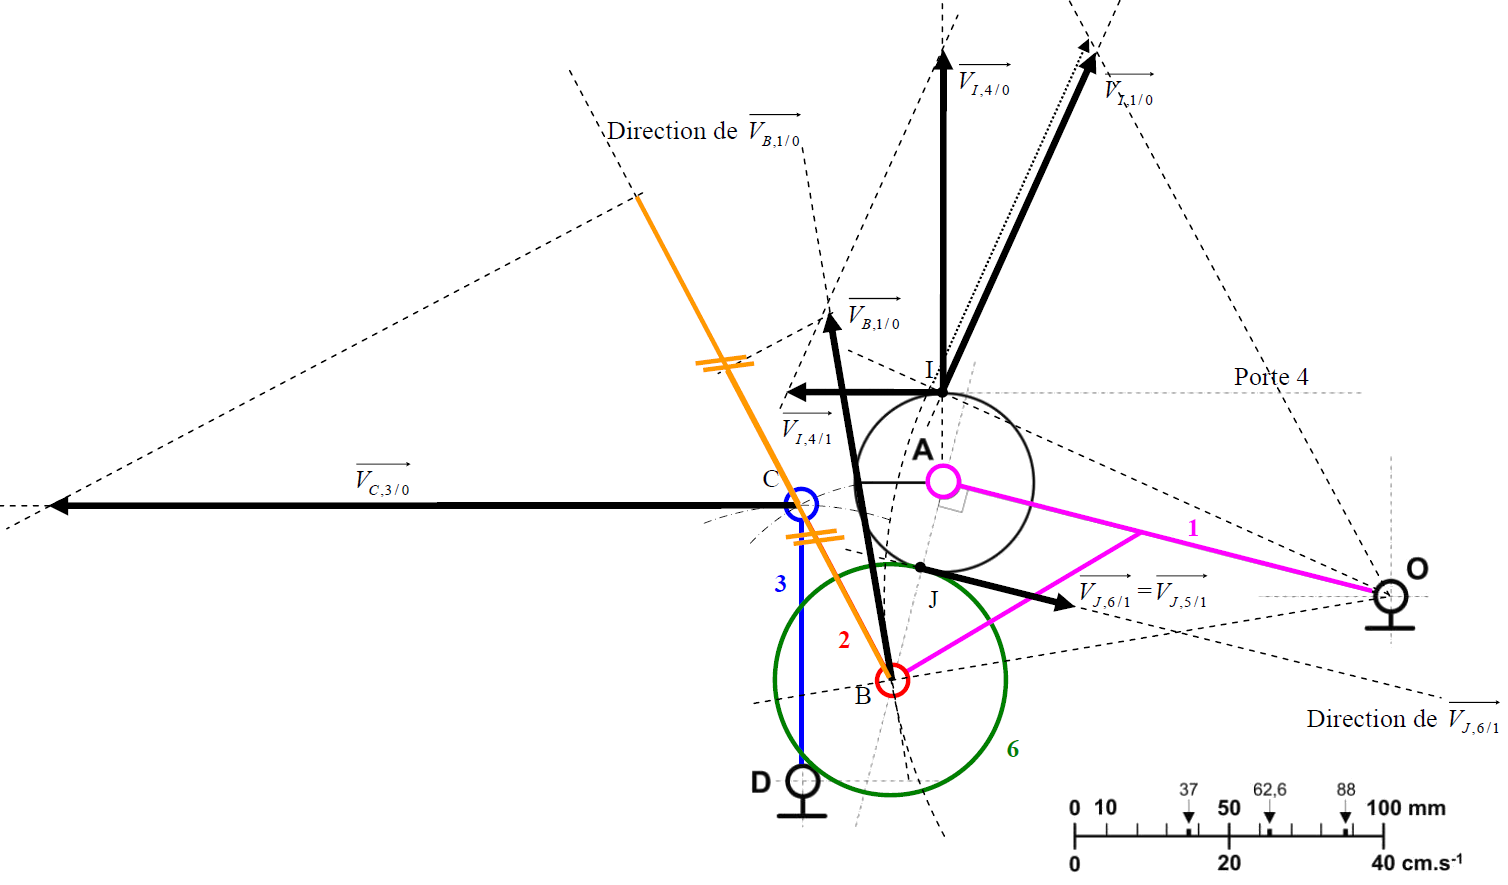
\includegraphics[width=\textheight]{images/cor_graphique}}
\end{center}
}{}

\subsection{Étude de la phase d'escamotage}
\ifthenelse{\boolean{prof}}{}{
On se place à présent dans la phase d’escamotage (cf. figure \ref{fig_05}) au cours de laquelle la position angulaire du bras support (1) par rapport à (0) reste celle atteinte par ce solide en fin de la phase de décalage. On observe le même comportement pour les solides (2) et (3). 
}

\ifthenelse{\boolean{prof}}{}{
\begin{figure}[!h]
\begin{center}
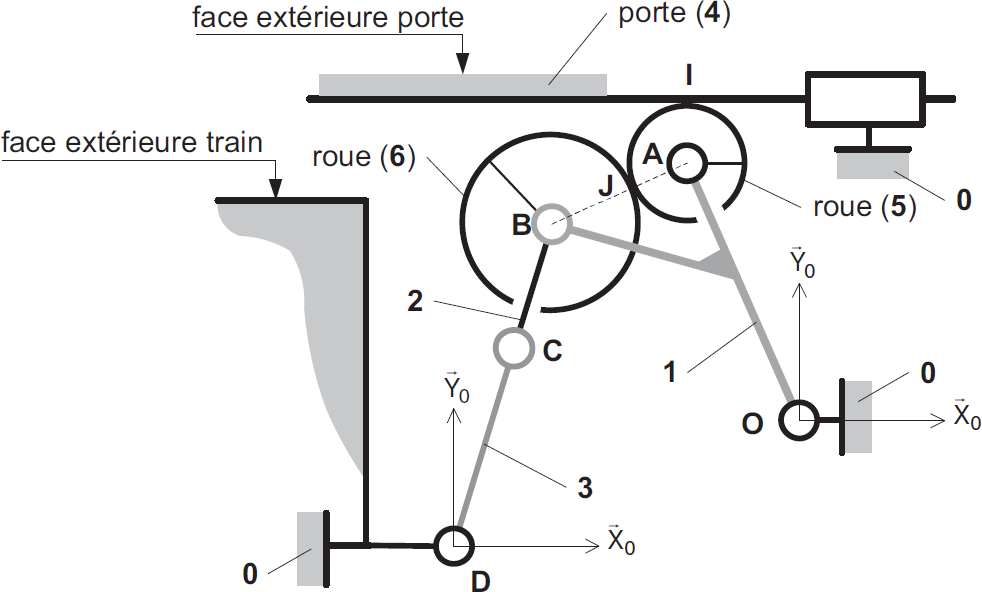
\includegraphics[width=.8\textwidth]{images/fig_07}

\caption{Schéma cinématique plan -- << Phase escamotage >> \label{fig_05}}
\end{center}
\end{figure}}


\subparagraph{}
\textit{Déterminer la valeur constante (en $mm$) de $\vect{OI}\cdot\vect{y_0}$ lors de la phase d’escamotage. Valider alors la satisfaction de l'exigence 8.2.3.}
\ifthenelse{\boolean{prof}}{
\begin{corrige}
Calculons $\vect{OI}\cdot\vect{y_0}$ : 
$$
\vect{OI}\cdot\vect{y_0} = \left(\vect{OA} + \vect{AI} \right)\cdot\vect{y_0}
= \vect{OA} \cdot\vect{y_0} + R_5 = L_1 \cos \theta_{10} + R_5
$$
$\theta_{10}=35\textdegree$ en fin de décalage. On a donc :
$$
\vect{OI}\cdot\vect{y_0} = 149 \cos 35 + 29 \simeq 151\; mm
$$

Par ailleurs $H_0 = 65,8 mm$ et l'épaisseur de la porte est de $40\; mm$. L'écart entre la porte et la face du train est donc de $151-40-65,8=45,2\; mm>40\; mm$. L'exigence est donc respectée. 

\end{corrige}}{}

\ifthenelse{\boolean{prof}}{}{
Afin de s’assurer d’une ouverture complète de la porte, on propose une loi de commande en vitesse du moteur. A l’instant initial, on suppose que $\dot{\theta}_m(t=0)=0$. Chronologiquement, la mise en rotation de l’actionneur s’effectue à accélération constante $\ddot{\theta_m}$ permettant d’atteindre, à l’instant $t_1$, la vitesse d’escamotage de la porte définie par le cahier des charges. Puis, à l’instant $t_2=2,8\; s$, une décélération constante permet d’atteindre à l’instant $t_3=3,1\; s$, une vitesse plus faible dite <<d’accostage>> définie par le cahier des charges. A l’instant $t_4=4\;s.$, la porte arrive en butée à la vitesse d’accostage assurant une ouverture complète.

Afin de garantir le temps d’ouverture, on utilise les valeurs maximales admissibles des vitesses d’escamotage et d’accostage définies par le cahier des charges. On suppose que les valeurs absolues des accélérations et des décélérations sont identiques et que toutes les liaisons sont parfaites.
}


%Q9.
\subparagraph{}
\textit{
%\begin{itemize}
%\item 
\`A partir de la description temporelle, tracer l’allure de la loi de commande en vitesse $\dot{\theta}_m(t)$ du moteur et la loi de commande en accélération $\dot{\theta}_m(t)$. Indiquer toutes les valeurs caractéristiques.
% Déterminer les valeurs (en $rd\cdot s^{-1}$) de $\dot{\theta}_m(t=t_1)$ et $\dot{\theta}_m(t=t_3)$.
%\item En utilisant le théorème de l’énergie cinétique, déterminer la valeur (en $rd.s^{-2}$) de l’accélération angulaire $\ddot{\theta}_m$ respectant la limitation de puissance consommée par le moteur électrique. Toutes les hypothèses nécessaires seront justifiées, les systèmes de solides isolés seront précisés et les différentes puissances seront exprimées avec rigueur. En déduire la valeur (en $s$) du temps $t_1$.
%\item Déterminer numériquement les temps $t_2$ et $t_3$ (en s) assurant une ouverture complète de la porte en $4\;s$.
%\end{itemize}
}

\ifthenelse{\boolean{prof}}{
\begin{corrige}
\begin{center}
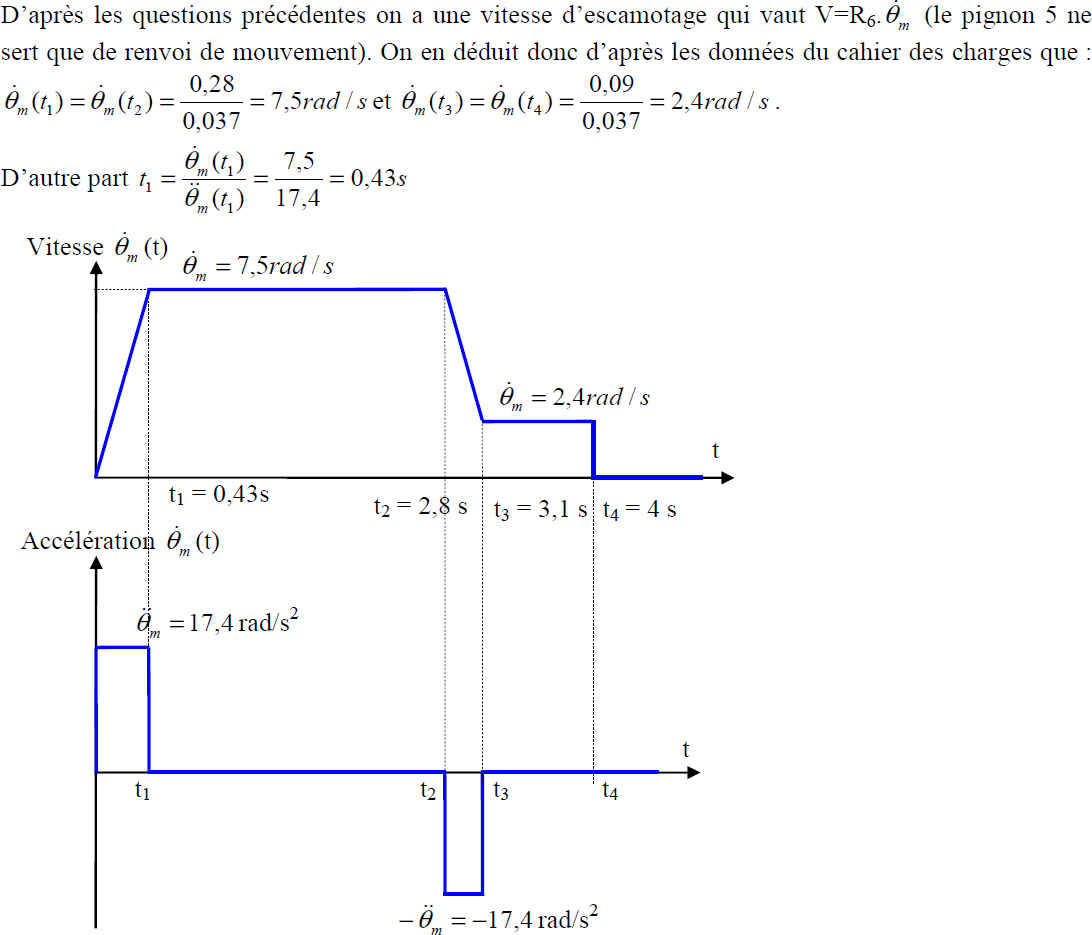
\includegraphics[width=.8\textwidth]{images/corr_courbes}
\end{center}
\end{corrige}}{}


\section{Étude de la commande de la porte en mode nominal}
\ifthenelse{\boolean{prof}}{}{
\begin{obj}
L’objectif est d’analyser le comportement du système piloté en chaîne directe et de valider la conformité avec le cahier des charges fonctionnel.
\end{obj}
}

\subsection{Analyse du modèle de commande de la porte}
\ifthenelse{\boolean{prof}}{}{
On se place uniquement dans la phase d’escamotage dont la durée moyenne est fixée à 4 s. La translation de la porte (4) le long de la caisse du train est notée $y_4(t)$. On fait l’hypothèse qu’à l’instant initial, correspondant au début de la phase d’escamotage étudiée, la porte est immobile avec $y_4(t=0)=0$ et $\theta_m(t=0)=0$. Grâce à une redéfinition du paramétrage et dans un soucis de simplification, on considère qu’au cours de cette phase $\omega_m(t) \geq 0$ et $y_4(t)\geq 0$.

  L’étude du moteur à courant continu commandé par l’induit assurant le déplacement de la porte donne les équations suivantes :
$$
u_m(t)=K_e\omega_m(t)+Ri_m(t) + L\dfrac{di_m(t)}{dt} \quad
\text{et}
\quad
 K_c i_m(t)-C_r(t) = J\dfrac{d\omega_m(t)}{dt}+f\omega_m(t)
$$

Les données du constructeur permettent d'obtenir les valeurs suivantes : 
$$
K_e = 0,86\; V\cdot s\cdot rad^{-1} 
\quad
K_c = 0,86\; Nm\cdot A^{-1}
\quad
R = 0,5\; \Omega
\quad
L=1\; mH
\quad
u_m\in [-24V;+24V]
$$

Le calcul de l’inertie équivalente de l’ensemble mobile en phase d’escamotage ramenée sur l’axe moteur mène au résultat suivant : $J=0,23\; kg\cdot m^2$ et on estime que $f=10^{-2} \, N\cdot m \cdot s \cdot rad^{-1}$.
On note  $\Omega_m(p)$ la transformée de Laplace de $\omega_m(t)$, $Y_4(p)$ la transformée de Laplace de $y_4(t)$, $\Theta_m(p)$ la transformée de Laplace de $\theta_m(t)$, $U_c(p)$ la transformée de Laplace de $u_c(t)$ …
La commande en chaîne directe de l’actionneur piloté en tension $u_c(t)$ peut être modélisée par le schéma bloc donné sur la figure \ref{fig_06}.

\begin{figure}[!h]
\begin{center}
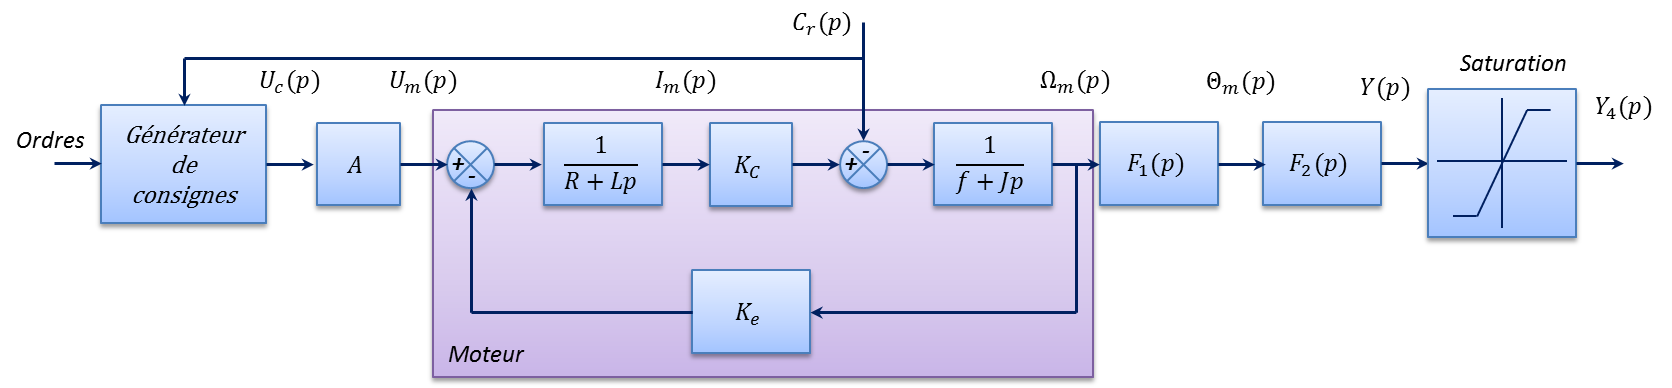
\includegraphics[width=\textwidth]{images/fig_08_bis}

\caption{Modèle de commande \label{fig_06}}
\end{center}
\end{figure}

La fonction de transfert de l’amplificateur de puissance est modélisée par un gain pur $A$ supposé unitaire.
}

\subparagraph{}
\textit{Montrer que la fonction de transfert du moteur non perturbé peut se mettre sous la forme  $\dfrac{\Omega_m(p)}{U_m(p)}=\dfrac{K_m}{\left(1+T_1p\right)\left(1+T_2p\right)}$. Déterminer l’expression du gain statique $K_m$. Déterminer les valeurs numériques (en s) des deux constantes de temps $T_1$ et $T_2$.}
\ifthenelse{\boolean{prof}}{
\begin{corrige}
On a : 
$$
\dfrac{\Omega_m(p)}{U_m(p)} 
= \dfrac{\dfrac{K_c}{(R+Lp)(f+Jp)}}{1+\dfrac{K_c K_e}{(R+Lp)(f+Jp)}}
= \dfrac{K_c}{(R+Lp)(f+Jp)+K_c K_e}
= \dfrac{K_c}{Rf+(Lf+RJ)p+LJp^2+K_c K_e}
$$
$$
= \dfrac{\dfrac{K_c}{Rf+K_cK_e}}{1+\dfrac{Lf+RJ}{Rf+K_cK_e}p+\dfrac{LJ}{Rf+K_cK_e}p^2}
$$

Par ailleurs, 
$$\dfrac{\Omega_m(p)}{U_m(p)}
=\dfrac{K_m}{\left(1+T_1p\right)\left(1+T_2p\right)}
=\dfrac{K_m}{1+T_1T_2p^2+\left(T_1+T_2\right)p}
$$

On a donc : 
$$
\dfrac{Lf+RJ}{Rf+K_cK_e} = T_1 + T_2 \quad \quad
\dfrac{LJ}{Rf+K_cK_e} = T_1 T_2
$$
\end{corrige}}{}



\ifthenelse{\boolean{prof}}{}{
On soumet le système (figure \ref{fig_06}) non perturbé à une entrée définie par $u_c(t)=u_0\cdot u(t)$ avec $u(t)$ : signal du type échelon unitaire, $u_0$ : tension en V. La réponse temporelle $y_4(t)$ est tracée sur la figure \ref{fig_07} pour trois valeurs distinctes de $u_0$.

\begin{figure}[!h]
\begin{center}
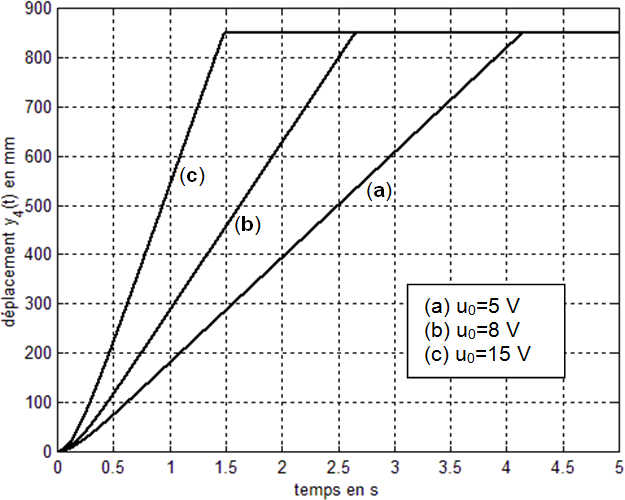
\includegraphics[width=.7\textwidth]{images/fig_09}

\caption{Réponse temporelle $y_4(t)$ \label{fig_07}}
\end{center}
\end{figure}
}

\subparagraph{}
\textit{En observant la figure \ref{fig_07}, proposer une description conditionnelle (si  …alors…) du bloc saturateur de la figure \ref{fig_06} en utilisant les variables $y_4(t)$ et $y(t)$. Quelle contrainte mécanique est modélisée par ce bloc ?}
\ifthenelse{\boolean{prof}}{
\begin{corrige}

Si $y(t)\leq850 \; mm$ alors $y_4(t)=y(t)$. 

Si $y(t)>850 \; mm$ alors $y_4(t)=850\; mm$.  

La saturation permet de prendre en compte la butée de fin de course. 
\end{corrige}}{}


\subparagraph{}
\textit{En vous aidant de la figure \ref{fig_07}, justifier le caractère non linéaire du saturateur.}
\ifthenelse{\boolean{prof}}{
\begin{corrige}
On observe que le comportement du saturateur n'est pas linéaire pour tout $t>0$. 
\end{corrige}}{}

%
%\subsection{Calibrage du système de commande}
%
%On cherche à calibrer un signal de commande plus conforme au cahier des charges et respectant un temps d’escamotage de 4 s. Après estimation et comparaison des différentes échelles de temps, on adopte le modèle simplifié suivant : le moteur se comporte comme un gain pur, soit $\Omega_m(p)=1,16\cdot U_m(p)$. On soumet le système de commande non perturbé à un signal défini par $u_c(t)=u_0 [u(t)-u(t-T)]$ avec $u(t)$ signal du type échelon unitaire, $u_0$ tension en $V$ et $T$ temps égal à 4 s.
%
%\subparagraph{}
%\textit{
%\begin{itemize}
%\item Tracer sur votre feuille l’allure temporelle du signal de commande $u_c(t)$ précédemment défini.
%\item Déterminer alors l’expression de $y_4(t)$ pour $0<t\leq T$. Quelle est la valeur de $y_4(t)$ pour $t>T$ ? En déduire la valeur de la tension $u_0$ (en V) satisfaisant le cahier des charges.
%\item Compléter alors le tracé en superposant en couleur l'allure complète de $y_4(t)$. Indiquer les valeurs remarquables déterminées précédemment. 
%\item Estimer la vitesse d’accostage de la porte (en $m\cdot s^{-1}$). Cette valeur est-elle conforme au cahier des charges fonctionnel ?
%\end{itemize}}
%
%En conservant les hypothèses consenties précédemment, on affine la forme du signal de commande $u_c(t)$ dont l’allure est précisée sur la figure \ref{fig_08}. On note $u_{10}$ et $u_{20}$ les deux niveaux distincts de tension (avec $u{10}>u_{20}$), $\Delta t$ le temps de maintien après accostage avant arrêt de l’alimentation du moteur à $t=t_f$. Ce temps est fixé à $\Delta t = 0,5\; s$.
%
%\begin{figure}[!h]
%\begin{center}
%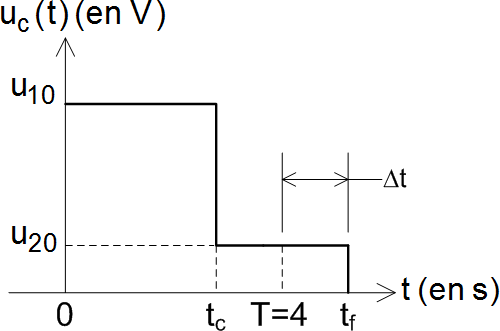
\includegraphics[width=.4\textwidth]{images/fig_10}
%
%\caption{Définition du signal de commande $u_c(t)$ \label{fig_08}}
%\end{center}
%\end{figure}
%
%
%\subparagraph{}
%\textit{
%\begin{itemize}
%\item En utilisant les conclusions de la question précédente, justifier en quelques lignes la forme du nouveau signal de commande $u_c(t)$ présentant cette fois un double niveau de tension.
%\item Déterminer la valeur (en V) des deux tensions $u_{10}$ et $u_{20}$ permettant de satisfaire les valeurs maximales admissibles (vitesse d’escamotage et vitesse d’accostage) définies par le cahier des charges fonctionnel.
%\item Déterminer alors la valeur de $t_c$ (en s) permettant d’obtenir une ouverture complète de la porte en $4\;s$.
%\item Tracer alors l’allure de l’évolution temporelle de $y_4(t)$. Placer les points remarquables, notamment $y_4(t=t_c)$ dont la valeur (en mm) sera déterminée.
%\end{itemize}}
%
%\subsection{Analyse de l'influence du couple résistant}
%
%On cherche à présent à quantifier l’influence du couple résistant $C_r(t)$ sur les performances de la commande. Le signal de commande $u_c(t)$ est de la forme définie par la figure \ref{fig_08}. Pour les questions suivantes, on suppose que $C_r(t)=C_{r0}\cdot u(t)$ avec $u(t)$ : signal du type échelon unitaire, $C_{r0}$ : amplitude du couple résistant en $N.m$.
%
%\subparagraph{}
%\textit{L’intensité et la vitesse de rotation du moteur s’établissent très rapidement comparativement à l’évolution globale. En négligeant les termes dérivés dans les équation fournies, la fonction de transfert simplifiée du moteur perturbé peut s’exprimer sous la forme $\Omega_m(p)=K_m\cdot U_m(p)-K_p\cdot C_r(p)$. Déterminer l’expression du gain $K_p$ et donner sa valeur numérique en précisant l’unité.}
%
%\subparagraph{}
%\textit{Montrer qu’en conservant les valeurs numériques des tensions $u_{10}$ et $u_{20}$ déterminées précédemment, si $C_{r0}>0$ alors $y_4(t=T)<850\; mm$ . Conclure quant à la capacité de cette structure de commande à respecter l’ensemble des critères du cahier des charges fonctionnel.}
%
%Afin de garantir le même niveau de performances de la commande malgré la présence du couple perturbateur, il est nécessaire d’adapter le signal de commande $u_c(t)$ et en particulier les nouvelles valeurs des tensions notées $\hat{u_{10}}$ et $\hat{u_{20}}$.
%
%
%\subparagraph{}
%\textit{
%\begin{itemize}
%\item Montrer que $\hat{u}_{10}=K\cdot C_{r0}+u_{10}$ et $\hat{u}_{20}=K\cdot C_{r0}+u_{20}$, $K\in \mathbb{R}$. Déterminer l’expression de $K$ en fonction de $K_m$ et   $K_p$;
%\item Déterminer la valeur maximale de $C_{r0}$ (en N.m) compatible avec la tension admissible aux bornes du moteur électrique.
%\end{itemize}}
%
%En toute rigueur, le temps lié à la mise en rotation du moteur n’est pas totalement négligeable. Il est impératif d’affiner le modèle de commande simplifié précédemment défini (Q14). Le générateur de consigne est réglé en conséquence et la figure \ref{fig_09} présente l’évolution temporelle du déplacement $y_4(t)$ et de la vitesse $\dot{y_4}(t)$.
%
%\begin{figure}[!h]
%\begin{center}
%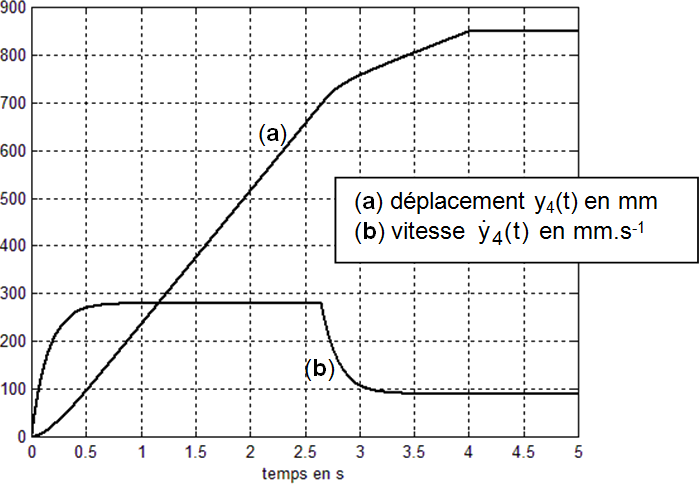
\includegraphics[width=.8\textwidth]{images/fig_11}
%
%\caption{Évolution temporelle de $y_4(t)$ et de $\dot{y_4}(t)$ \label{fig_09}}
%\end{center}
%\end{figure}
%
%\subparagraph{}
%\textit{\begin{itemize}
%\item Indiquer de manière qualitative, les différences notables entre votre tracé (Q13d) et la figure \ref{fig_09}. Dans quelles zones observe-t-on ces différences ?
%\item Le générateur de consigne ainsi réglé nous permet-il de valider le cahier des charges fonctionnel ?
%\end{itemize}}

\subsection{Estimation du couple résistant}

%Nous avons montré que le respect du cahier des charges au cours du cycle d’utilisation du système d’ouverture était assujetti au calibrage correct de la loi de commande étudiée précédemment. 
\ifthenelse{\boolean{prof}}{}{
Afin de respecter le cahier des charges, il est nécessaire d'avoir une estimation du couple résistant $C_r(t)$. Or l’évolution de cette grandeur en fonctionnement n’est pas accessible directement par un capteur contrairement au courant de l’induit $i_m(t)$ et de la fréquence de rotation du moteur $\omega_m(t)$.
 
 Il est cependant possible de reconstruire une information (estimation) sur la valeur du couple résistant (notée $\hat{C}_r(t)$) grâce à une chaîne qui utilise des grandeurs issues de mesures effectuées directement sur l’ensemble variateur-moteur ( $i_m(t)$ et $\omega_m(t)$ ). La figure \ref{fig_10} donne l’architecture de cette chaîne.


\begin{figure}[!h]
\begin{center}
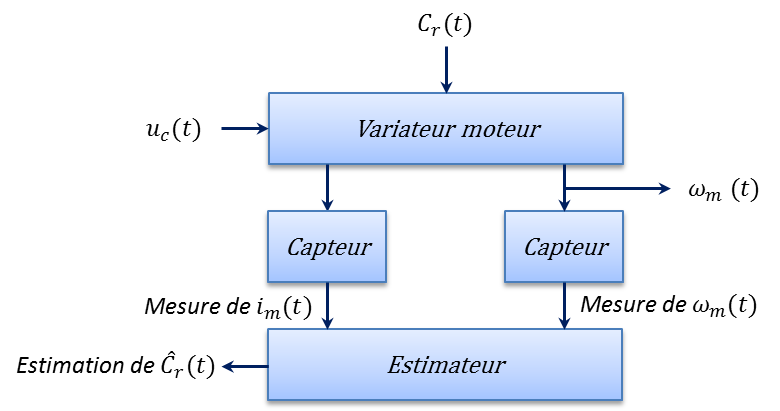
\includegraphics[width=.6\textwidth]{images/fig_12_bis}

\caption{Architecture de la chaîne d’estimation \label{fig_10}}
\end{center}
\end{figure}

Une modélisation de cette architecture réelle est cependant indispensable pour concevoir l’estimateur. On suppose que la chaîne décrite précédemment se réduit au schéma bloc suivant (cf. figure \ref{fig_11}).

\begin{figure}[!h]
\begin{center}
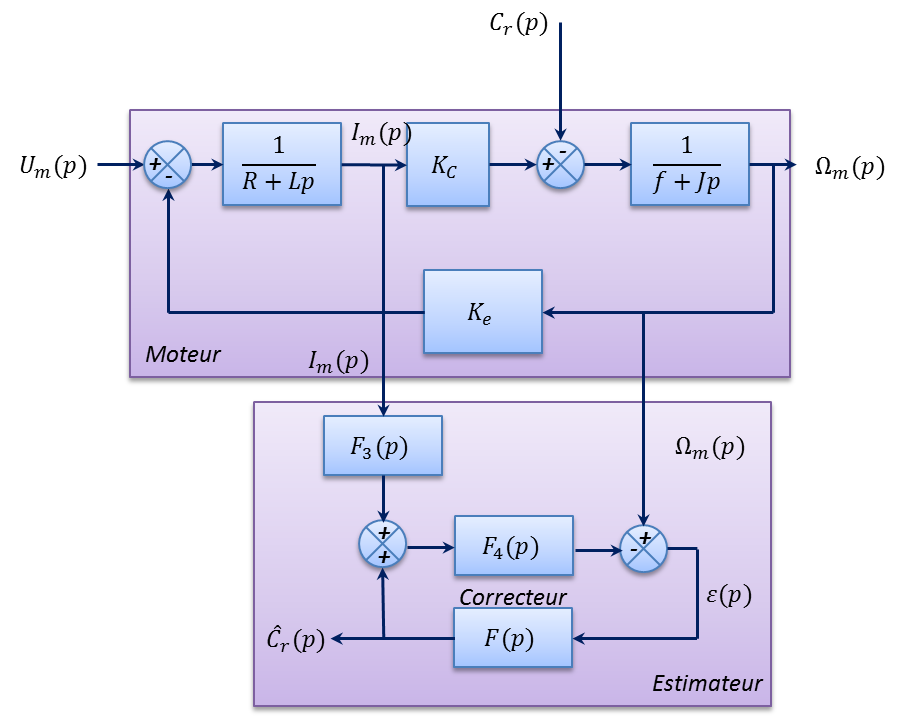
\includegraphics[width=.75\textwidth]{images/fig_13_bis}

\caption{Schéma bloc du moteur et de l’estimateur \label{fig_11}}
\end{center}
\end{figure}

On note $\hat{C}_r(t)$ l'estimation du couple résistant et F(p) la fonction de transfert du correcteur. En toute rigueur $I_m(p)$ et $\Omega_m(p)$ représentent des grandeurs mesurées directement sur le système réel.

L’objectif est de construire un estimateur qui nous permette de nous ramener à un problème d'asservissement où la consigne est la grandeur de perturbation $C_r(p)$ et la sortie sa valeur estimée $\hat{C}_r(p)$.

Pour obtenir une bonne estimation, l’estimateur doit être précis et rapide.

Le cahier des charges est le suivant :
\begin{itemize}
\item erreur en position nulle : $\varepsilon_p (\infty) = C_r(\infty)-\hat{C}_r(\infty) = 0$;
\item erreur de traînage inférieure à 1\% ;
\item temps de réponse à 5\% inférieur à 0,05 s.
\end{itemize}
}

\subparagraph{}
\textit{D'après le schéma bloc du moteur, déterminer $\Omega_m(p)$ en fonction de $C_r(p)$ et $I_m(p)$.}
\ifthenelse{\boolean{prof}}{
\begin{corrige}
On a directement :
$$
\Omega_m(p) = \left(K_c I_m(p) - C_r(p)\right)\cdot\dfrac{1}{f+Jp}
$$
\end{corrige}}{}


\subparagraph{}
\textit{D'après le schéma bloc de l'estimateur, déterminer $\varepsilon(p)$ en fonction de $\Omega_m(p)$, $\hat{C}_r(p)$ et $I_m(p)$ et déterminer $\hat{C}_r(p)$ en fonction de $\varepsilon(p)$.}
\ifthenelse{\boolean{prof}}{
\begin{corrige}
On a : 
$$
\varepsilon(p) = \Omega_m(p)-\left(I_m(p)\cdot F_3(p)+\hat{C}_r(p) \right)F_4(p)
$$

Par ailleurs :
$$
\hat{C}_r(p) = F(p)\varepsilon(p)
$$
\end{corrige}}{}


\subparagraph{}
\textit{En déduire la relation entre $\hat{C}_r(p)$, $C_r(p)$ et $I_m(p)$. Déterminer $F_3(p)$ et $F_4(p)$ afin que l'estimateur puisse se mettre sous la forme du schéma bloc figure \ref{fig_12}.}
\ifthenelse{\boolean{prof}}{
\begin{corrige}
On a d'une part :
$$
\hat{C}_r(p) 
= \dfrac{\dfrac{F(p)}{f+Jp}}{1+\dfrac{F(p)}{f+Jp}} C_r(p) 
= \dfrac{F(p)}{f+Jp+F(p)} C_r(p) 
$$

Par ailleurs :
$$
\dfrac{\hat{C}_r(p)}{F(p)} = \left( K_cI_m(p) - C_r(p)\right)\cdot\dfrac{1}{f+Jp}-\left(I_m(p)\cdot F_3(p)+\hat{C}_r(p) \right)F_4(p)
$$
$$
\Longleftrightarrow 
\hat{C}_r(p) = \left(K_c I_m(p) - C_r(p)\right)\cdot\dfrac{F(p)}{f+Jp}-F(p)\left(I_m(p)\cdot F_3(p)+\hat{C}_r(p) \right)F_4(p)
$$
$$
\Longleftrightarrow 
\hat{C}_r(p)\left(1+F(p)F_4(p)\right) = \left(K_c I_m(p) - C_r(p)\right)\cdot\dfrac{F(p)}{f+Jp}-\left(I_m(p)\cdot F_3(p)\right)F(p)F_4(p)
$$

$$
\Longleftrightarrow 
\hat{C}_r(p)\left(1+F(p)F_4(p)\right) = \dfrac{F(p)}{f+Jp}K_c I_m(p) -\dfrac{F(p)}{f+Jp} C_r(p)-F(p)\cdot F_3(p)F_4(p)I_m(p)
$$
$$
\Longleftrightarrow 
\hat{C}_r(p) = \left(\dfrac{K_c}{f+Jp} - F_3(p)F_4(p)\right)\dfrac{F(p)}{1+F(p)F_4(p)}I_m(p)-\dfrac{F(p)}{\left(f+Jp\right)\left(1+F(p)F_4(p)\right)} C_r(p)
$$

Pour pouvoir se mettre sous la forme du schéma bloc donné, il faut donc que :
$$
\dfrac{K_c}{f+Jp} - F_3(p)F_4(p) = 0
$$

Par identification, on a donc $F_3(p)=K_c$ et $F_4(p)=\dfrac{1}{f+Jp}$.
\end{corrige}}{}


\ifthenelse{\boolean{prof}}{}{
\begin{figure}[!h]
\begin{center}
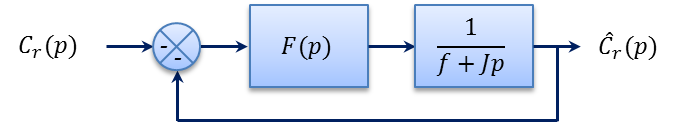
\includegraphics[width=.6\textwidth]{images/fig_14_bis}

\caption{Schéma bloc équivalent \label{fig_12}}
\end{center}
\end{figure}

On choisit le correcteur suivant $F(p)=K_{cor} \dfrac{1+T_{cor}\cdot p}{T_{cor} p}$.
}

%\subparagraph{}
%\textit{Comment appelle-t-on ce correcteur ? Par rapport à l’emploi d’un correcteur proportionnel, pourquoi permet-il d'avoir une estimation de $C_r$ plus précise ?}

\subparagraph{}
\textit{Quel doit être le gain statique en boucle fermée de la fonction de transfert de l’estimateur afin que l'erreur en position soit nulle ? Est-ce le cas ?}
\ifthenelse{\boolean{prof}}{
\begin{corrige}
On souhaite par ailleurs que :
$$
\underset{t\to \infty}{\lim} \varepsilon_p (t) = \underset{t\to \infty}{\lim} C_r(t)-\hat{C}_r(t) = 0 
\Longrightarrow 
\underset{p\to 0}{\lim} \varepsilon_p (p) =\underset{p\to 0}{\lim} p( C_r(p)-\hat{C}_r(p))= 0 
$$

On a :
$$
\dfrac{\hat{C}_r(p)}{C(p)} 
= \dfrac{K_{cor} \dfrac{1+T_{cor}\cdot p}{T_{cor} p}}{f+Jp+K_{cor} \dfrac{1+T_{cor}\cdot p}{T_{cor} p}}
= \dfrac{K_{cor} (1+T_{cor}\cdot p)}{fT_{cor} p+JT_{cor} p^2+K_{cor} (1+T_{cor}\cdot p)}
= \dfrac{1+T_{cor}\cdot p}{1+ T_{cor}(1+\dfrac{f}{K_{cor}} )p+ \dfrac{JT_{cor}}{K_{cor}} p^2}
$$

La FTBF a donc un gain unitaire et tend donc bien vers 1 lorsque $p$ tend vers 0.


\end{corrige}}{}

On donne $T_{cor}=\dfrac{J}{f}$ et $K_{cor}=10$.

\subparagraph{}
\textit{Tracer en vert les diagrammes de Bode (asymptotiques et réels) de la fonction de transfert en boucle ouverte de l’estimateur sans correcteur. Faire apparaître les points caractéristiques.}
\ifthenelse{\boolean{prof}}{
\begin{corrige}
\begin{center}
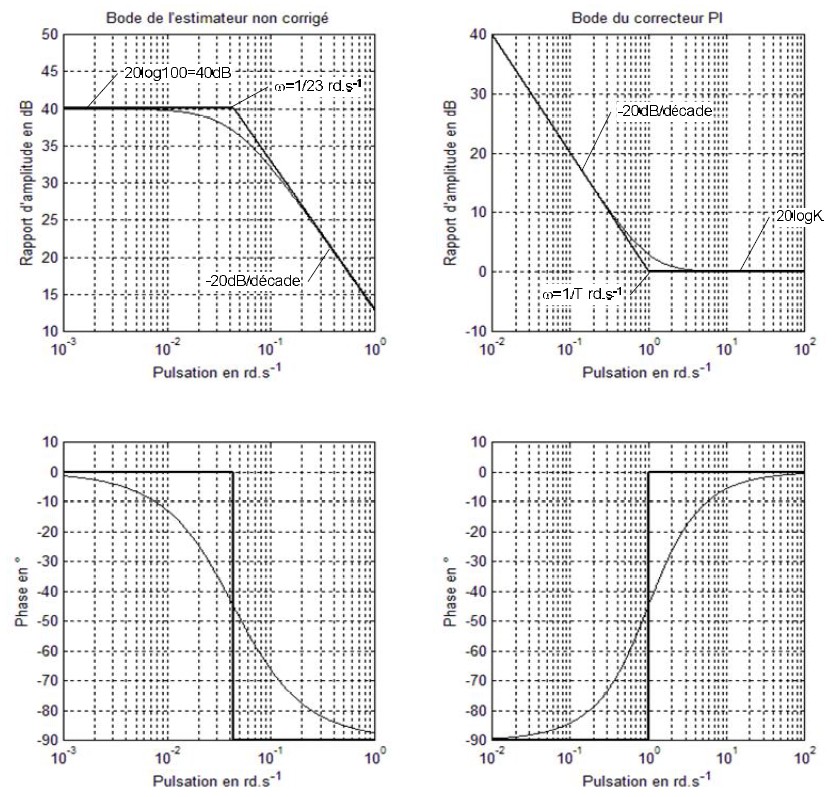
\includegraphics[width=.6\textwidth]{images/corr_bode}
\end{center}
\end{corrige}}{}



\subparagraph{}
\textit{Tracer en rouge les diagrammes de Bode (asymptotiques et réels) du correcteur. Faire apparaître les points caractéristiques.}

On rappelle que $J=0,23\; kg\cdot m^2$ et que $f=10^{-2}\, N\cdot m \cdot s \cdot rad^{-1}$ .

%\subparagraph{}
%\textit{On cherche à régler le correcteur. Déterminer $T_{cor}$ afin que le zéro du correcteur compense le pôle de l’estimateur non corrigé. Faire l’application numérique.}

\subparagraph{}
\textit{Déterminer $K_{cor}$  pour vérifier l’erreur de traînage imposée par le cahier des charges. Faire l’application numérique.}
\ifthenelse{\boolean{prof}}{
\begin{corrige}

L'erreur du système est donnée par : 
$$
\varepsilon(p) = C_r(p) \cdot \dfrac{1}{1+K_{cor} \dfrac{1+T_{cor}\cdot p}{T_{cor} p}\cdot\dfrac{1}{f+Jp} }
 =  C_r(p) \dfrac{T_{Cor}p(f+Jp)}{T_{Cor}p(f+Jp)+K_{cor}(1+T_{cor}p)}
$$
L'erreur de trainage se calcule à partir d'une entrée en rampe (de pente $a$): $C_r(p)=\dfrac{a}{p^2}$.

On a donc 
$$
\varepsilon_v 
= \underset{p\to 0}{\lim} p \cdot \dfrac{a}{p^2} \cdot  \dfrac{T_{Cor}p(f+Jp)}{T_{Cor}p(f+Jp)+K_{cor}(1+T_{cor}p)}
= \underset{p\to 0}{\lim} \dfrac{T_{Cor}a(f+Jp)}{T_{Cor}p(f+Jp)+K_{cor}(1+T_{cor}p)}
=\dfrac{T_{cor}af}{K_{cor}}
$$

Prenons une pente de 1.
$ \varepsilon_v  = \dfrac{T_{cor}f}{K_{cor}}<0,01 \Longleftrightarrow K_{cor} > 100 f T_{cor} \Longleftrightarrow K_{cor} > 23$.
\end{corrige}}{
}

\subparagraph{}
\textit{On donne les tracés de la réponse indicielle (entrée unitaire) de la fonction de transfert de en boucle fermée de l’estimateur avec et sans correction. Faire apparaître sur chaque tracé l’erreur de position et le temps de réponse à 5\%.
Vérifie-t-on tous les critères du cahier des charges de l’estimateur ?
}
\begin{center}
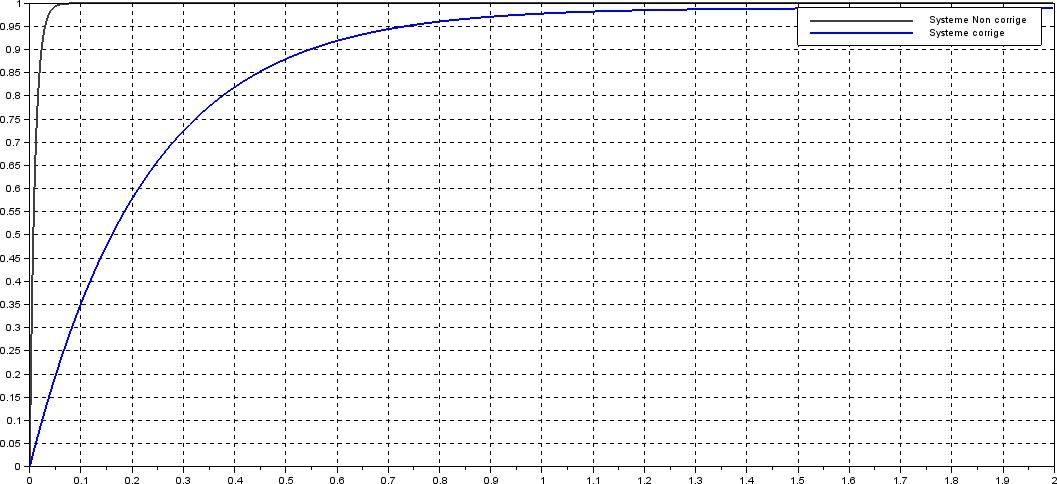
\includegraphics[width=.6\textwidth]{images/corr_rep_temp}
\end{center}
\ifthenelse{\boolean{prof}}{
\begin{corrige}
Le système corrigé répond à l'exigence d'écart statique nul et de temps de réponse inférieur à 0,05 seconde (0,01 seconde).
\end{corrige}}{}


\end{document}


